\documentclass[10pt, landscape]{article}
\usepackage[scaled=0.92]{helvet}
\usepackage{calc}
\usepackage{multicol}
\usepackage{ifthen}
\usepackage[a4paper,margin=3mm,landscape]{geometry}
\usepackage{amsmath,amsthm,amsfonts,amssymb}
\usepackage{color,graphicx,overpic}
\usepackage{hyperref}
\usepackage{newtxtext} 
\usepackage{enumitem}
\usepackage{amssymb}
\usepackage[table]{xcolor}
\usepackage{vwcol}
\usepackage{tikz}
\usetikzlibrary{arrows.meta}
\usetikzlibrary{calc}
\usepackage{mathtools}
\usepackage{nicematrix}
%For pictures / figures
\usepackage{color,graphicx,overpic}
\graphicspath{ {./images/} }
% for relations
\usepackage{cancel}
\usepackage{ mathrsfs }
\graphicspath{ {./images/} }
\setlist{nosep}
\usepackage{amssymb}  % For \checkmark


\pdfinfo{
  /Title (CG2271-Final-Cheatsheet.pdf)
  /Creator (TeX)
  /Producer (pdfTeX 1.40.0)
  /Author (Seamus)
  /Subject (Example)
  /Keywords (pdflatex, latex,pdftex,tex)}

% Turn off header and footer
\pagestyle{empty}

\newenvironment{tightcenter}{%
  \setlength\topsep{0pt}
  \setlength\parskip{0pt}
  \begin{center}
}{%
  \end{center}
}

% redefine section commands to use less space
\makeatletter
\renewcommand{\section}{\@startsection{section}{1}{0mm}%
                                {-1ex plus -.5ex minus -.2ex}%
                                {0.5ex plus .2ex}%x
                                {\normalfont\large\bfseries}}
\renewcommand{\subsection}{\@startsection{subsection}{2}{0mm}%
                                {-1explus -.5ex minus -.2ex}%
                                {0.5ex plus .2ex}%
                                {\normalfont\normalsize\bfseries}}
\renewcommand{\subsubsection}{\@startsection{subsubsection}{3}{0mm}%
                                {-1ex plus -.5ex minus -.2ex}%
                                {1ex plus .2ex}%
                                {\normalfont\small\bfseries}}%
\renewcommand{\familydefault}{\sfdefault}
\renewcommand\rmdefault{\sfdefault}
% makes nested numbering (e.g. 1.1.1, 1.1.2, etc)
\renewcommand{\labelenumii}{\theenumii}
\renewcommand{\theenumii}{\theenumi.\arabic{enumii}.}
\renewcommand\labelitemii{•}
%  for logical not operator
\renewcommand{\lnot}{\mathord{\sim}}
\renewcommand{\bf}[1]{\textbf{#1}}
\newcommand{\abs}[1]{\vert #1 \vert}
\newcommand{\Mod}[1]{\ \mathrm{mod}\ #1}

\makeatother
\definecolor{myblue}{cmyk}{1,.72,0,.38}
\everymath\expandafter{\the\everymath \color{myblue}}
% Define BibTeX command
\def\BibTeX{{\rm B\kern-.05em{\sc i\kern-.025em b}\kern-.08em
    T\kern-.1667em\lower.7ex\hbox{E}\kern-.125emX}}
\let\iff\leftrightarrow
\let\Iff\Leftrightarrow
\let\then\rightarrow
\let\Then\Rightarrow

% Don't print section numbers
\setcounter{secnumdepth}{0}

\setlength{\parindent}{0pt}
\setlength{\parskip}{0pt plus 0.5ex}
%% this changes all items (enumerate and itemize)
\setlength{\leftmargini}{0.5cm}
\setlength{\leftmarginii}{0.5cm}
\setlist[itemize,1]{leftmargin=2mm,labelindent=1mm,labelsep=1mm}
\setlist[itemize,2]{leftmargin=4mm,labelindent=1mm,labelsep=1mm}

%My Environments
\newtheorem{example}[section]{Example}
% -----------------------------------------------------------------------

\begin{document}
\raggedright
\footnotesize
\begin{multicols}{4}


% multicol parameters
% These lengths are set only within the two main columns
\setlength{\columnseprule}{0.25pt}
\setlength{\premulticols}{1pt}
\setlength{\postmulticols}{1pt}
\setlength{\multicolsep}{1pt}
\setlength{\columnsep}{2pt}

\begin{center}
    \fbox{%
        \parbox{0.8\linewidth}{\centering \textcolor{black}{
            {\Large\textbf{CG2271 Final}}
            \\ \normalsize{AY26/27 sem 1}}
            \\ {\footnotesize \textcolor{myblue}{github.com/mendax1234}} 
        }%
    }
\end{center}

\section{Intro to OS}
\begin{enumerate}
    \item OS is nothing special but a program which does
    \begin{itemize}
        \item virtualization of CPU via context switch and scheduling; virtualization of memory via giving each process a private address space
        \item solving the issues related to concurrency
        \item storing files persistently.
    \end{itemize}
    % \item MIPS Instructions table: \\
    % %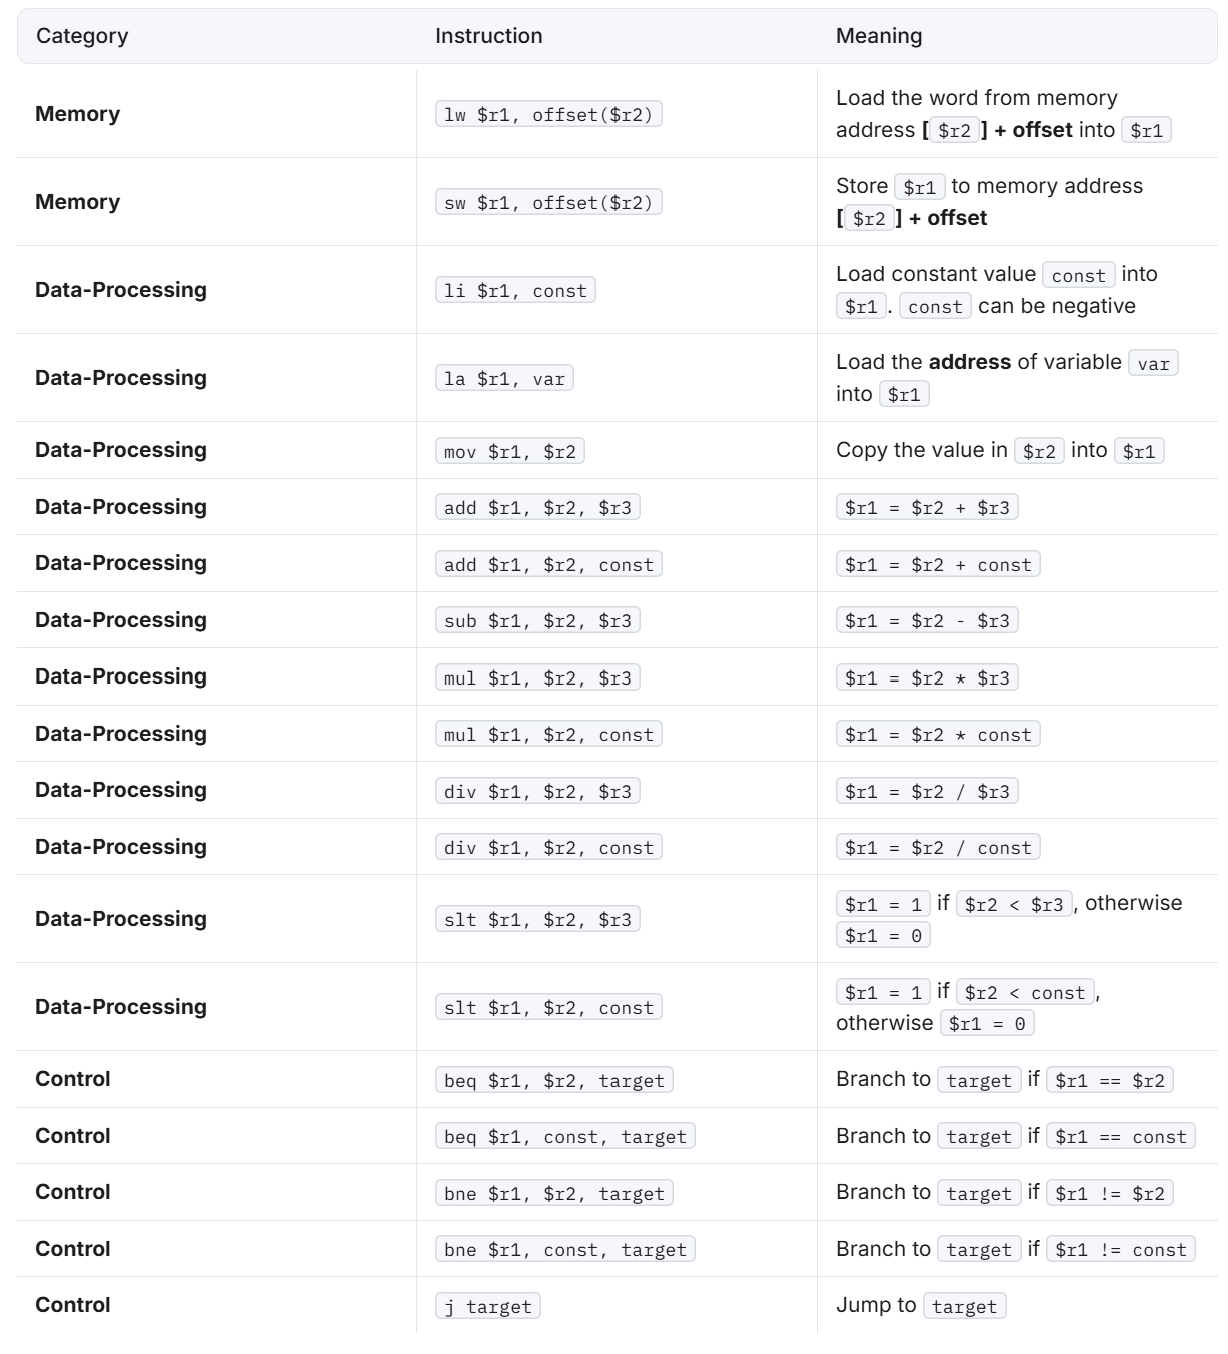
\includegraphics[width=1\linewidth]{images/midterm/2.png}
    % {\centering
    % \footnotesize
    % \setlength{\tabcolsep}{2.5pt}
    % \renewcommand{\arraystretch}{1.1}
    % \begin{tabular}{l p{0.45\columnwidth}}
    % \hline
    % \textbf{Instruction} & \textbf{Meaning} \\
    % \hline
    % \texttt{lw \$r1, offset(\$r2)} & Load word from \textbf{[\texttt{\$r2}] + offset} into \texttt{\$r1} \\
    % \texttt{sw \$r1, offset(\$r2)} & Store \texttt{\$r1} to \textbf{[\texttt{\$r2}] + offset} \\
    % \hline
    % \texttt{li \$r1, const} & Load constant \texttt{const} into \texttt{\$r1} (can be negative) \\
    % \texttt{la \$r1, var} & Load address of \texttt{var} into \texttt{\$r1} \\
    % \texttt{mov \$r1, \$r2} & Copy \texttt{\$r2} into \texttt{\$r1} \\
    % \texttt{add \$r1, \$r2, \$r3} & \texttt{\$r1 = \$r2 + \$r3} \\
    % \texttt{add \$r1, \$r2, const} & \texttt{\$r1 = \$r2 + const} \\
    % \texttt{sub \$r1, \$r2, \$r3} & \texttt{\$r1 = \$r2 - \$r3} \\
    % \texttt{mul \$r1, \$r2, \$r3} & \texttt{\$r1 = \$r2 * \$r3} \\
    % \texttt{mul \$r1, \$r2, const} & \texttt{\$r1 = \$r2 * const} \\
    % \texttt{div \$r1, \$r2, \$r3} & \texttt{\$r1 = \$r2 / \$r3} \\
    % \texttt{div \$r1, \$r2, const} & \texttt{\$r1 = \$r2 / const} \\
    % \texttt{slt \$r1, \$r2, \$r3} & \texttt{\$r1 = 1} if \texttt{\$r2 < \$r3}, else \texttt{0} \\
    % \texttt{slt \$r1, \$r2, const} & \texttt{\$r1 = 1} if \texttt{\$r2 < const}, else \texttt{0} \\
    % \hline
    % \texttt{beq \$r1, \$r2, tgt} & Branch to \texttt{tgt} if \texttt{\$r1 == \$r2} \\
    % \texttt{beq \$r1, const, tgt} & Branch to \texttt{tgt} if \texttt{\$r1 == const} \\
    % \texttt{bne \$r1, \$r2, tgt} & Branch to \texttt{tgt} if \texttt{\$r1 != \$r2} \\
    % \texttt{bne \$r1, const, tgt} & Branch to \texttt{tgt} if \texttt{\$r1 != const} \\
    % \texttt{j tgt} & Jump to \texttt{tgt} \\
    % \hline
    % \end{tabular}\par}
    % \begin{itemize}
    %     \item For control instructions, \texttt{target} usually refers to a label, which identifies the location to jump or branch to.
    %     \item \texttt{lw} is used to read a variable's value from memory into a register, e.g., \texttt{lw \$1, x} is used to load the variable \texttt{x}'s value into register 1. After modifying the value, \texttt{sw} is used to write the updated value back to memory.
    %     \item The usual flow for writing a decision in assembly is:
    %     \begin{enumerate}
    %         \item Set up the condition check, usually using \texttt{slt}.
    %         \item Branch to the \texttt{else} part if the condition is false.
    %         \item Execute the \texttt{if} part if the condition is true and remember to jump to skip the else part.
    %         \item Continue after the else part using another label.
    %     \end{enumerate}
    % \end{itemize}
    \item Variables declared \textbf{outside} \texttt{main()} are \textbf{global variables}, so they are stored in the \textbf{data memory region}.
    \item (\textbf{Monolithic Structure}): Since almost everything is in kernel mode, this structure has very \textbf{good performance}, but it is dangerous. \\
    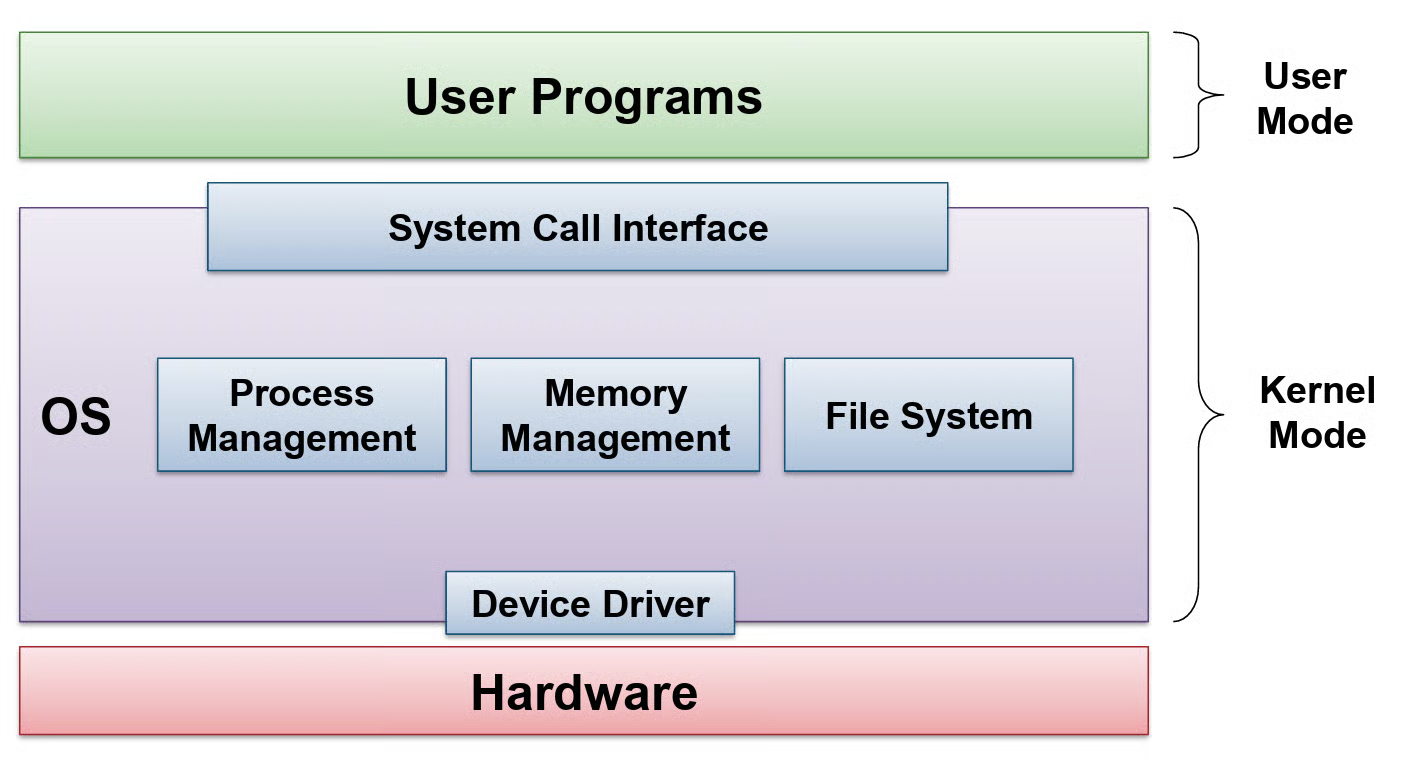
\includegraphics[width=1\linewidth]{images/midterm/4.png}
    \item (\textbf{Microkernel Structure}): All the higher level services are separate out, making the programs running in kernel mode very \textbf{small and clean}. However, the disadvantage is \textbf{low performance} as we need frequent context switches. \\
    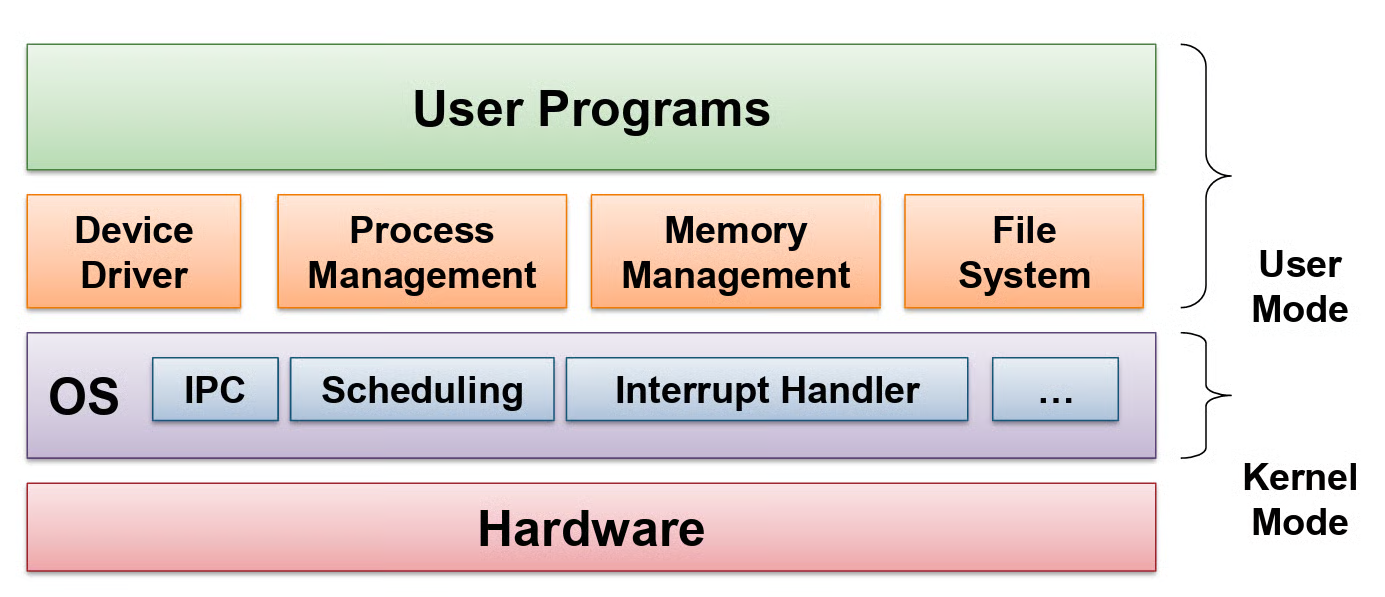
\includegraphics[width=1\linewidth]{images/midterm/5.png}
    \begin{itemize}
        \item It is \textbf{wrong} to say that in a monolithic OS, the entire kernel is compiled as a single large program.
        \item Microkernel OSes provide IPC mechanism to allow communication between programs in user mode and kernel mode.
        \item Process scheduler runs in \textbf{kernel mode} in both monolithic and microkernel OSes!
    \end{itemize}
    \item \textbf{ISR:} handles hardware interrupts and notifies the OS of events (e.g.\ I/O completion), allowing waiting processes to move \textbf{Blocked $\rightarrow$ Ready}.
    \item \textbf{OS:} virtualizes/abstracts hardware for processes.
    \item \textbf{Hypervisor:} virtualizes hardware for multiple \textbf{guest operating systems / VMs}.
    \item \textbf{Types of VMs}: Type 1 hyperviser sits on top of the \textbf{hardware} while type 2 hypervisor sits on top of a \textbf{host OS}.
    \item \textbf{Attention:} Uninitialized local variables read residual (dirty) values from whichever prior frame data shared that exact stack slot.
\end{enumerate}

\section{Process Abstraction}
\begin{enumerate}
    \item The machine state of a process contains the following 3 contexts which are stored in the \textbf{process control block (PCB)} (except for memory context)
    \begin{itemize}
        \item Memory Context: Code, Data, Stack, Heap. PCB does \textbf{not} store actual memory contents (Code, Data, Heap, Stack). PCB stores \textbf{memory-management information/pointers} needed to locate and manage the process's address space.
        \item Hardware Context: Registers, PC, $\dots$
        \item OS Context: Process Properties, Resources used
    \end{itemize}
    \item Each process has its own address space, namely memory context.
    \item (\textbf{User Stack}): The user stack is a region of memory used to store information associated with function calls. Each function invocation is represented by a stack frame.
    \item (\textbf{User Stack Pointer}): This pointer always points to the top of the user stack for a given process.
    \item In C, it is impossible for a callee to access the variables in the caller that are not passed to callee!
    \item (\textbf{Frame pointer}): A frame pointer always points to the bottom (start) of the current stack frame, making it easier to access the local variables and arguments passed from the caller because their offsets from the frame pointer remain fixed.
    \item (\textbf{Process Table}): The Process Table can be thought of as a data structure maintained by the kernel that contains an entry for every process. \textbf{Each entry is a PCB}, which is why a PCB is also referred to as a \textbf{process table entry (PTE)}.
    \item The process table and PCB both reside in \textbf{kernel space}, while the process's actual memory space resides in \textbf{user space}.
    \item Typically, to calculate the stack frame's size when calling a function, we should consider:
    \begin{itemize}
        \item \textbf{Return address / PC}: where execution resumes.
        \item \textbf{Saved old FP}: restores caller's frame pointer.
        \item \textbf{Saved old SP}: if required by the calling convention.
        \item \textbf{Parameters}: if passed on the stack.
        \item \textbf{Local variables}: variables declared inside the function.
        \item \textbf{Return-value space}: if stored on the stack.
        \item \textbf{Saved registers}: temporary registers that must be preserved.
    \end{itemize}
    \item A calling convention that allocates a fixed 4 bytes per parameter/local does \textbf{not} support arbitrary data types. To support any type, allocate stack space according to each variable's \textbf{size and alignment}; large objects may be passed by pointer.
    \item A calling convention example:\par
    {\centering
    \begin{tabular}{ll}
    \hline
    \textbf{Value stored} & \textbf{Location} \\
    \hline
    Saved old FP & $FP$ \\
    Saved old SP & $FP+4$ \\
    Return address & $FP+8$ \\
    Parameter 1 & $FP+12$ \\
    Parameter 2 & $FP+16$ \\
    $\vdots$ & $\vdots$ \\
    Parameter $n$ & $FP+4(n+3)$ \\
    Return value & $FP+4(n+4)$ \\
    Start of local-variable area & $FP+4(n+5)$ \\
    Local variables & $FP+4(n+5)$ to $SP$ \\
    \hline
    \end{tabular}\par}
    \begin{itemize}
        \item \textbf{Caller} allocates the basic frame up to $FP+4(n+5)$.
        \item \textbf{Callee} extends $SP$ by $4m$ bytes to reserve space for its local variables. ($m$ denotes the number of local variables)
    \end{itemize}
    \item (\texttt{fork()}): When a process calls \texttt{fork()}, the OS creates a new process by copying the parent process's PCB, including its hardware, OS, and memory contexts. The OS context is then updated with a new PID, while the child continues executing the same code from the point immediately after \texttt{fork()}.
    \begin{itemize}
        \item A successful call to \texttt{fork()} always \textbf{doubles} the number of executing processes. (The problem of ``fork-bomb'').
        \item The return value of \texttt{fork()} differs between the parent and child process:
        \begin{itemize}
            \item Child process: \texttt{fork()} returns 0.
            \item Parent process: \texttt{fork()} returns the \textbf{PID} ($>$0) of the newly created child.
            \item \textbf{\texttt{-1}}: Indicates failure; no child is created, and \texttt{errno} is set.
        \end{itemize}
        \item After each \texttt{fork()}, the parent and child have separate copies of their \textbf{local and global variables}. Changes to these variables in one process do not affect the other, allowing each process to maintain independent state.
    \end{itemize}
    \item \texttt{exec()}: Usually called by a child process after \texttt{fork()} to replace its current program (code, data, heap, and stack) with a new program, while retaining the same PID.
    \item \texttt{wait()}: Usually called by a parent process to block until one of its child processes terminates. Returns the terminated child's PID (e.g., \texttt{int wc = wait(NULL);}).
    \item (\textbf{Process State Transition}): \\
    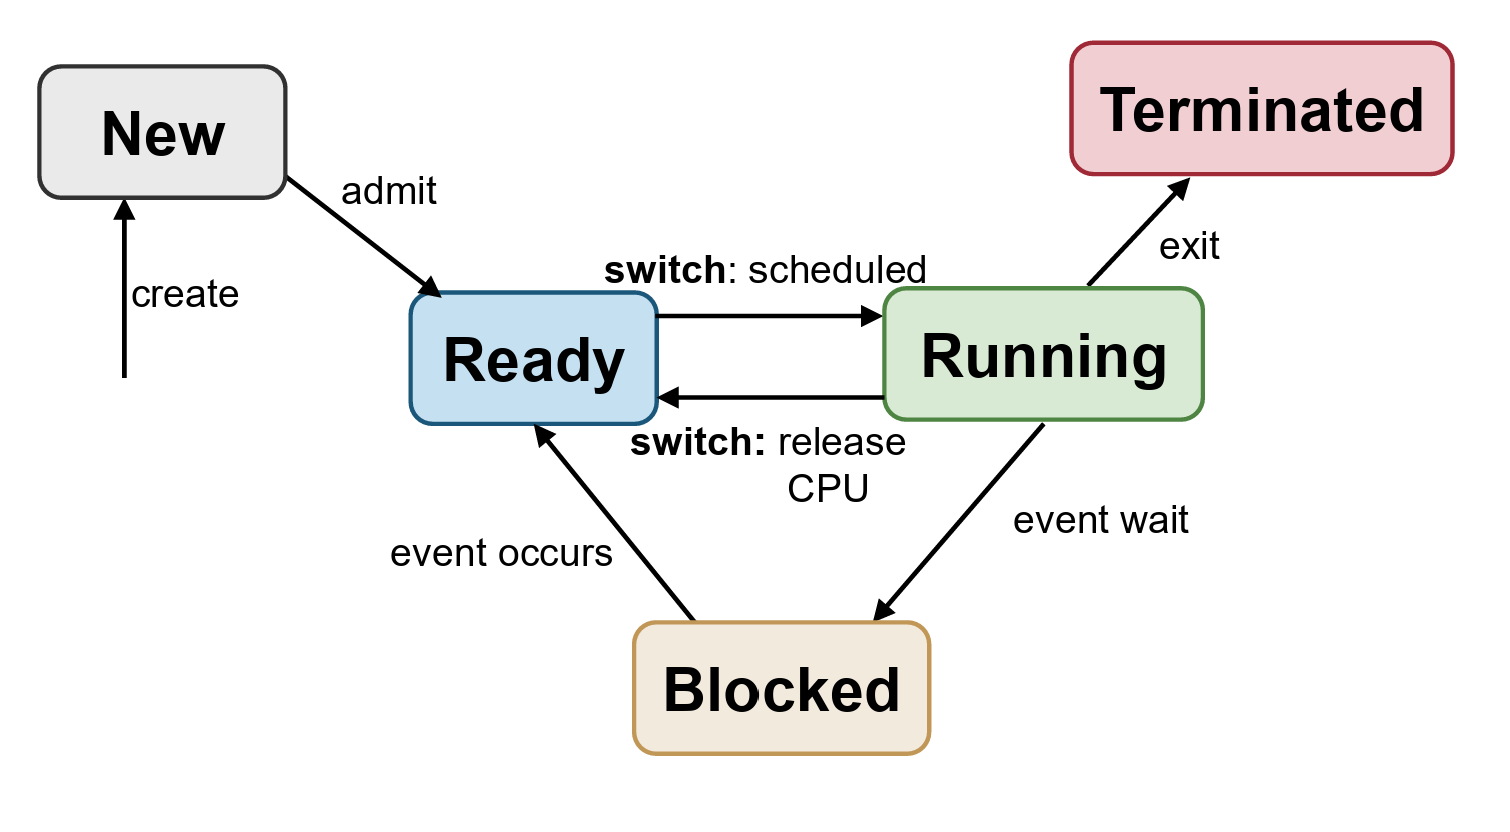
\includegraphics[width=1\linewidth]{images/midterm/7.png}
\end{enumerate}

\section{Process Scheduling}
\begin{enumerate}
    \item (\textbf{Turnaround time}): $T_{\text{turnaround}}=T_{\text{completion}}-T_{\text{arrival}}$
    \item (\textbf{Response time}): $T_{\text{response}}=T_{\text{firstrun}}-T_{\text{arrival}}$
    \item (\textbf{RTOS Scheduling}): RTOS scheduling can be classified by how task priorities are assigned. We normally assume \textbf{pre-emption is enabled} and \textbf{time-slicing is disabled}.
    \begin{itemize}
        \item \textbf{Fixed-Priority Scheduling}: Each task is assigned a fixed priority that does not change.
        \item \textbf{Rate Monotonic Scheduling (RMS)}: A fixed-priority scheme where priority is determined by the task's \textbf{period}; a shorter period gives a higher priority.
        \item \textbf{Earlier Deadline First (EDF)} scheduling: This is not a fixed priority scheduling scheme, a task's priority is increased as its deadline approaches.
        \item If CPU utilization is under 100\%, EDF always guarantees schedulability.
        \item \textbf{Deadlines}: A task's deadline is the \textbf{latest time by which it must finish}. In periodic real-time tasks, the deadline is often equal to the task's \textbf{period}, meaning one instance should finish before the next instance is released.
    \end{itemize}
    \item (\textbf{Liu and Layland Bound}: This is to check if a set of tasks is schedulable under RMS. A set of $n$ periodic tasks is guaranteed to be schedulable under RMS if $U \leq n\left(2^{1/n}-1\right)$, where $U=\sum_i\frac{C_i}{P_i}$. Tasks that fail to meet L\&L bound may still be schedulable under RMS.
    \item (\textbf{Critical Instance Analysis}): It tests the schedulability systematically by computing the worst-case response time of each task.
    \begin{itemize}
        \item Sort the tasks by period: If the tasks are not already sorted, arrange them in increasing order of period. Thus, $T_1$ has the shortest period, $T_2$ the second shortest, and so on.
        \item For each task $T_i$, recursively compute $S_{i,0}, S_{i,1}, \ldots$
        \item $S_{i,0} = \sum_{j=1}^{i} C_j$: This represents the initial workload when all higher-priority tasks and $T_i$ are released simultaneously.
        \item $S_{i,x+1} = C_i + \sum_{j=1}^{i-1} \left\lceil \frac{S_{i,x}}{P_j} \right\rceil C_j$: The summation accounts for the preemptions caused by higher-priority tasks. Continue until $S_{i,x+1} = S_{i,x}$ and call this final value $S_{i,F}$. ($x+1$ can be greater than $i$)
        \item Check the deadline: $S_{i,F} \le D_i$. If this condition holds for every task $T_i$, then the entire task set is schedulable under RMS and no task will miss its deadline.
        \item (\textbf{Tips}): Usually we start with the \textbf{lowest-priority task} first. But to check a set of tasks is schedulable, we need to verify each task is schedulable.
    \end{itemize}
    \item \textbf{Example: Critical Instant Analysis (RMS)}
    \begin{tabular}{c|cc}
    \hline
    \textbf{Task} & \textbf{Period }$P_i$ & \textbf{Execution Time }$C_i$ \\
    \hline
    $T_1$ & 6 & 2 \\
    $T_2$ & 8 & 2 \\
    $T_3$ & 4 & 1 \\
    \hline
    \end{tabular}
    
    \begin{itemize}
        \item Under RMS, sort by increasing period:
              $\{T_3,T_1,T_2\}$, so $T_2$ is the \textbf{lowest-priority task}.
        \item \textbf{Check $T_2$:}
        \[
        S_{2,0}=C_3+C_1+C_2=1+2+2=5
        \]
        \[
        S_{2,1}=C_2+\left\lceil\frac{5}{4}\right\rceil C_3
        +\left\lceil\frac{5}{6}\right\rceil C_1
        =2+2+2=6
        \]
        \[
        S_{2,2}=2+\left\lceil\frac{6}{4}\right\rceil(1)
        +\left\lceil\frac{6}{6}\right\rceil(2)=6
        \]
        Since $S_{2,2}=S_{2,1}=6\leq P_2=8$, $T_2$ is schedulable.
    \end{itemize}
    \item (\textbf{Pre-emptive} Priority Scheduling): In this scheme, don't use the idea of ready queue, if need, the ready queue is prioritized!
    \item In this course, we made the following conventions when scheduling tasks (Please refer to the actual Test)
    \begin{itemize}
        \item A task arriving at time $x$ becomes ready exactly at time $x$ (on the horizontal axis), as illustrated below.
        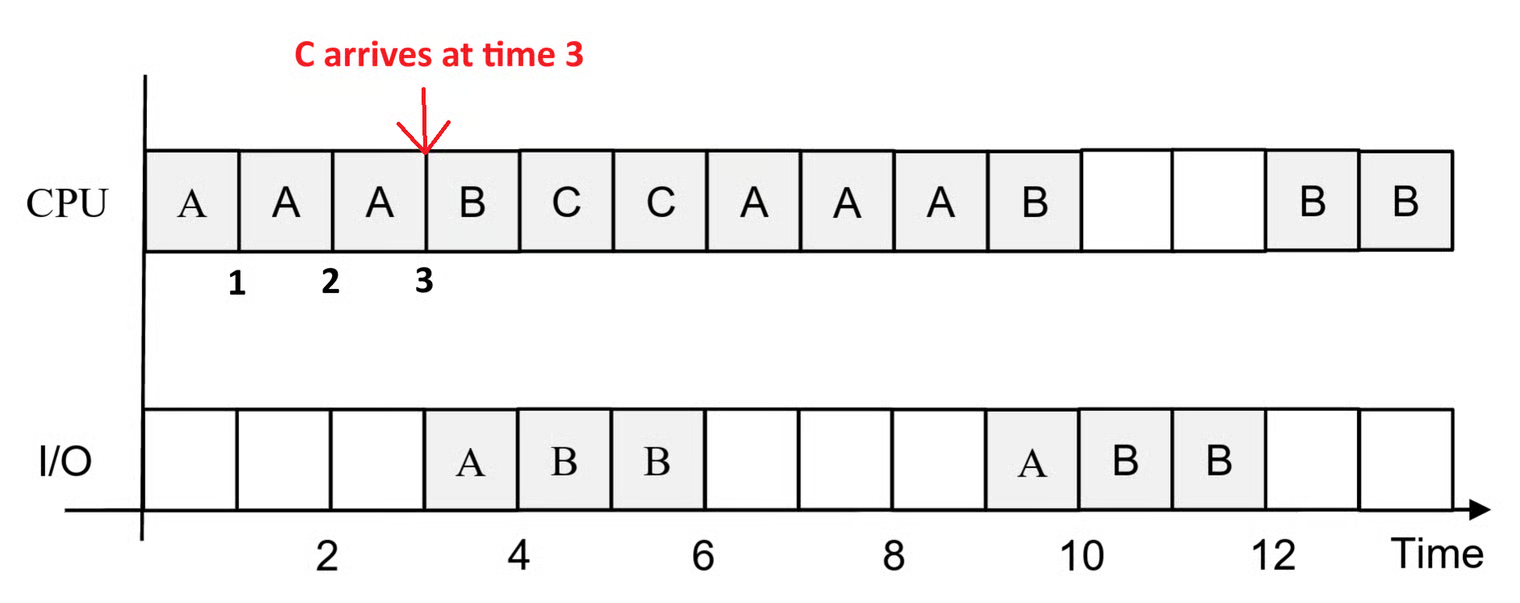
\includegraphics[width=1\linewidth]{images/midterm/3.png}
        \item When calculating turnaround time, use the R.H.S coordinates. When calculating the response time, use the L.H.S coordinates. for the scheduling above, assume B arrives at time 1.
        \begin{tabular}{c|cc}
        \hline
        \textbf{Process} & \textbf{Turnaround Time} & \textbf{Response Time} \\
        \hline
        A & 9  & 0 \\
        B & 13 & 2 \\
        C & 3  & 1 \\
        \hline
        \end{tabular}
    \end{itemize}
    
    \item (\textbf{Waiting Time}): $\text{Waiting Time}=\text{Turnaround Time}-\text{Service Time}$, where service time is the total time during which the task is actually running on the CPU or I/O.
    \item (\textbf{Round Robin} Scheduling): 
    \begin{itemize}
        \item If a process finishes before its time quantum expires, immediately schedule another ready process and \textbf{the ready process will start a fresh new time quantum}; the CPU does \textbf{not} wait for the remaining quantum. CPU is idle only if the ready queue is empty.
        \item \textbf{Round Robin is preemptive by time quantum:} a new arrival does \textbf{not} preempt the running process merely because it has higher priority.
        \item \textbf{Round Robin (RR)} maintains a \textbf{FIFO ready queue}. Each ready process runs for at most a fixed \textbf{time quantum}. If the quantum expires and the process is not finished, it is \textbf{preempted} and moved to the \textbf{back of the ready queue}.
    \end{itemize}
    \item We must take the \textbf{I/O} completion time also into account when calculating the turnaround time and waiting time!
    \item (\textbf{Shortest Job First (SJF) Scheduling}): The scheduler will run the \textbf{shortest} job first, then the \textbf{next shortest}, and so on.
    \item When analyzing which scheduling algorithm is better, it's always a ``it depends'' question. So, one tip is to clearly compare the trade-off between turnaround time and response time.
\end{enumerate}

\section{Threads}
\begin{enumerate}
    \item Each thread has its own \textbf{hardware context}, which include registers and user stack (these user stacks will stay in the same stack memory region of the process, thus making the stack memory region fragmented).
    \begin{itemize}
        \item Each thread also has its own \textbf{thread-related OS context}: thread ID, state, priority, scheduling information, etc.
        \item Threads in the same process \textbf{share process-level OS resources} such as the address space and open files.
    \end{itemize}
    \item (\textbf{User Thread}): A user thread is implemented by a thread library in user space, so the kernel is not aware of individual threads and it only sees a process is running. The library and its runtime system manage thread creation, switching, and scheduling.
    \begin{itemize}
        \item Advantages: thread operations are fast because they are just library calls, the scheduling policy can be customized, and user threads can run on almost any OS.
        \item Disadvantages: because the kernel schedules at the process level, one blocked thread can block the entire process, and the process cannot exploit multiple CPUs by running its threads in parallel.
    \end{itemize}
    \item (\textbf{Kernel Thread}): A kernel thread is implemented and managed by the OS. Thread operations are handled through system calls, and the kernel can schedule individual threads. In other words, the kernel now has the knowledge of which thread within a process is runnable. \textbf{However}, the trade-off is that thread operations are more expensive because they require kernel involvement, and the implementation is generally less flexible.
    \item Threads are ``lightweight processes'' because they have \textbf{less creation/context-switch overhead} than full processes.
    \item Pthread API
        \begin{itemize}
        \item \texttt{pthread\_create(\&tid, NULL, func, arg)}: starts a thread running \texttt{func(arg)}.
        \item The \texttt{pthread\_create} returns 0 to indicate success and !0 to indicate errors.
        \item Thread function format: \texttt{void *func(void *arg)}.
        \item \texttt{pthread\_exit(ret)}: terminates the thread and returns \texttt{ret}.
        \item \texttt{pthread\_join(tid, \&ret)}: waits for the thread; stores the thread's return value in \texttt{ret}. This is called thread synchronization. Without it, the child thread might terminate when its parent process finishes executing. To let the parent process wait for its child, we should use this API.
        \item \texttt{pthread\_join()} itself returns \textbf{0 on success}, not the thread's return value.
    \end{itemize}
    \item When counting possible thread execution interleavings, remember that \textbf{statements within the same thread must preserve their original execution order}.
    \item \textbf{Race Condition (Interleavings)}:
    \begin{itemize}
        \item Break each read-modify-write operation into \textbf{Load + Compute} (combined, assuming local computation) and \textbf{Store}. (e.g., Process 1 can be L1A, S1A, L1B, S1B, process 2 can be L2A, S2A.)
        \item For $k$ processes with $n_1,n_2,\ldots,n_k$ ordered operations, the number of valid interleavings is $\frac{(n_1+n_2+\cdots+n_k)!}{n_1!n_2!\cdots n_k!}$.
        \item \textbf{Systematic Method}: Choose positions for each process sequentially, filling the remaining positions with the last process. Always preserve each process's internal order.
        \item Simulate the interleavings to find the \textbf{unique final values}, which may be fewer than the number of interleavings.
    \end{itemize}
\end{enumerate}

\section{Inter-Process Communication}
\begin{enumerate}
    \item (\textbf{Synchronization}): The send or receive operation blocks the process until the required communication can take place. For example
    \begin{itemize}
        \item The read process waits until the pipe is not empty then it will start reading.
        \item The write process waits until the pipe is not full when it will start writing.
    \end{itemize}
    \item \textbf{Shared-memory race:} processes created by \texttt{fork()} can access the same shared-memory object. If multiple processes write the same location without synchronization, the final value is \textbf{non-deterministic}.
    \item Shared Memory API:
    \begin{itemize}
    \item \texttt{shmid = shmget(key, size, flags)}: create/get a shared-memory segment $\rightarrow$ \texttt{shmid}.
    \begin{itemize}
        \item \texttt{key}: identifies the shared-memory segment.
        \item \texttt{size}: allocate space for $N$ elements using \texttt{N * sizeof(type)}.
        \item \texttt{flags}: e.g.\ \texttt{IPC\_CREAT | 0600}; \texttt{0} indicates octal notation, and \texttt{6 = rw-} gives the owner read/write permission while the two \texttt{0}s give group and others no permission. If we use hex, it will be \texttt{0x180}.
    \end{itemize}
        \item \texttt{shm = shmat(shmid,...)}: attaches a shared-memory segment to a pointer in user space so that we can use the pointer to access the shared memory. The shared-memory segment itself is managed by the kernel and thus living in the kernel space.
        \begin{itemize}
            \item After attach, can use \texttt{shm[0,$\dots$,N-1]} to access the value in the shared memory region if we want to create an array in the shared memory region.
        \end{itemize}
        \item Access shared memory normally through the returned pointer.
        \item \texttt{shmdt(ptr)}: detach shared memory.
        \item \texttt{shmctl(shmid, IPC\_RMID, NULL)}: delete shared-memory segment.
    \end{itemize}
    \item (\textbf{UNIX Pipe}):
    \begin{itemize}
        \item Pipe ends: \texttt{fd[0]} = read, \texttt{fd[1]} = write.
        \item Writer closes \texttt{fd[0]}; reader closes \texttt{fd[1]}.
        \item Empty pipe + write end still open $\Rightarrow$ \textbf{read blocks}.
        \item Empty pipe + all write ends closed $\Rightarrow$ \textbf{EOF}.
        \item Full pipe + blocking \texttt{write()} $\Rightarrow$ writer blocks; data is not simply lost.
        \item \texttt{dup2(fd[0], STDIN\_FILENO)} redirects \texttt{stdin} from the keyboard to the \textbf{pipe read end}.
        \item \texttt{dup2(fd[1], STDOUT\_FILENO)} redirects \texttt{stdout} from the screen to the \textbf{pipe write end}.
    \end{itemize}
\end{enumerate}

\section{Synchronization}
\begin{enumerate}
    \item \textbf{Semaphore Behaviour}:
    \begin{itemize}
        \item \texttt{wait(S)}: If $S \leq 0$, block; otherwise, $S \gets S-1$.
        \item \texttt{signal(S)}: $S \gets S+1$; wake up a waiting process, if any.
    \end{itemize}
    Thus, the process will be blocked \textbf{before} the semaphore gets decreased. When a process is blocked by calling \texttt{wait(Semaphore)}, it must wait for another process/thread to call \texttt{signal(Semaphore)}. This may wake the blocked process, allowing it to continue executing its \texttt{wait()} operation and decrement the semaphore before continuing execution.
    \item Deadlock can occur when processes acquire multiple semaphores in different orders, causing each process to wait for a resource held by the other. \\ 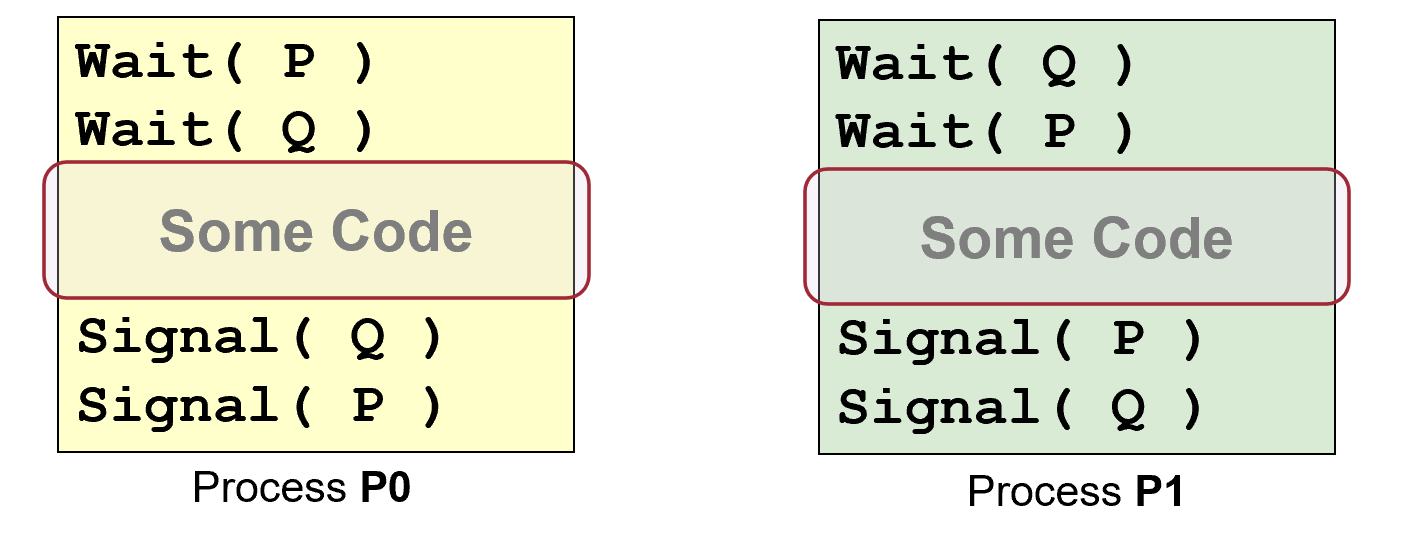
\includegraphics[width=1\linewidth]{images/midterm/1.png}
    \item The beauty of using semaphores is that it allows the thread \textbf{blocked to sleep} instead of \textbf{busy waiting} and consume the CPU resources uselessly.
    \item Binary semaphores are commonly used for mutual exclusion, while counting semaphores are used to track the number of available resources/conditions and block threads when none are available. For example, in the producer-consumer problem, we solve it using three semaphores:
    \begin{itemize}
        \item mutex = 1: ensures mutual exclusion when accessing the buffer.
        \item notFull = K: number of empty slots available.
        \item notEmpty = 0: number of items available to consume.
    \end{itemize}
    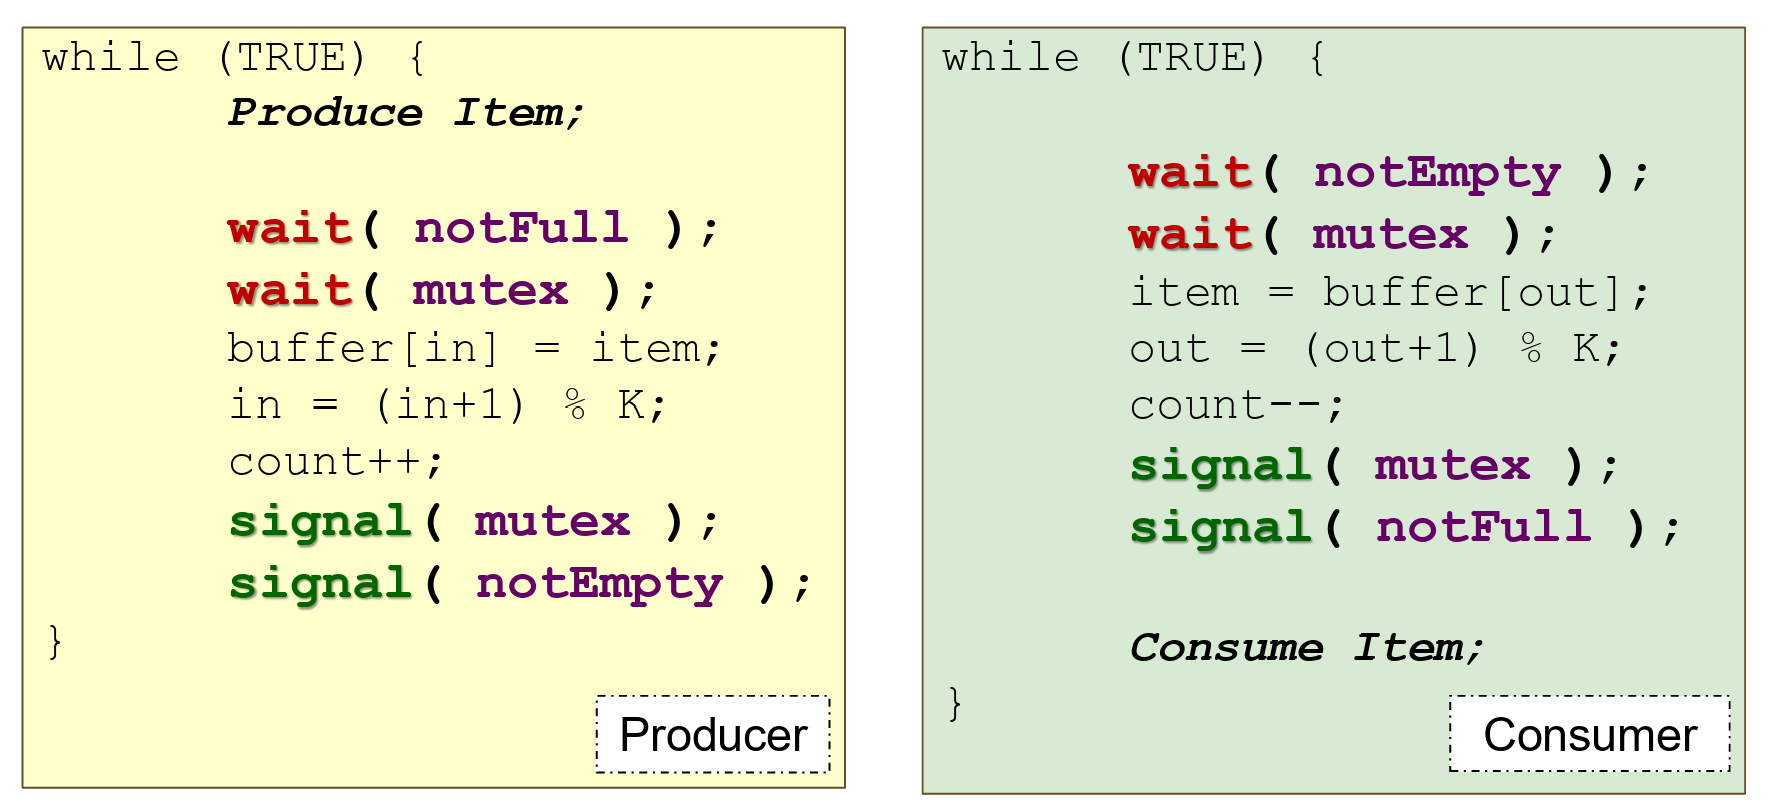
\includegraphics[width=1\linewidth]{images/final/14.png}
    \item Operations that modify the state or value of a semaphore or mutex are performed atomically. The critical section doesn't need to be executed atomically!
    \item When analyzing the correctness of a solution using semaphores, always consider the \textbf{starvation} can be possible or not!
\end{enumerate}

\section{Memory Abstraction}
\begin{enumerate}
    \item \textbf{Two principles of locality}
    \begin{itemize}
        \item \textbf{Temporal Locality}: If we have used a piece of data recently, we are likely to use it again soon.
        \item \textbf{Spatial Locality}: When we use one particular piece of data, we are likely to be interested in other pieces of data in the same area.
    \end{itemize}
    \item Physical addresses specify where data actually resides, while logical addresses specify where a process thinks its data resides.
    \item \textbf{External fragmentation} occurs as processes are created, terminated, or swapped out. Even if the total free memory is sufficient, a new process may not fit because no individual hole is large enough.
    \item When doing buddy system, draw the following diagram: \\
    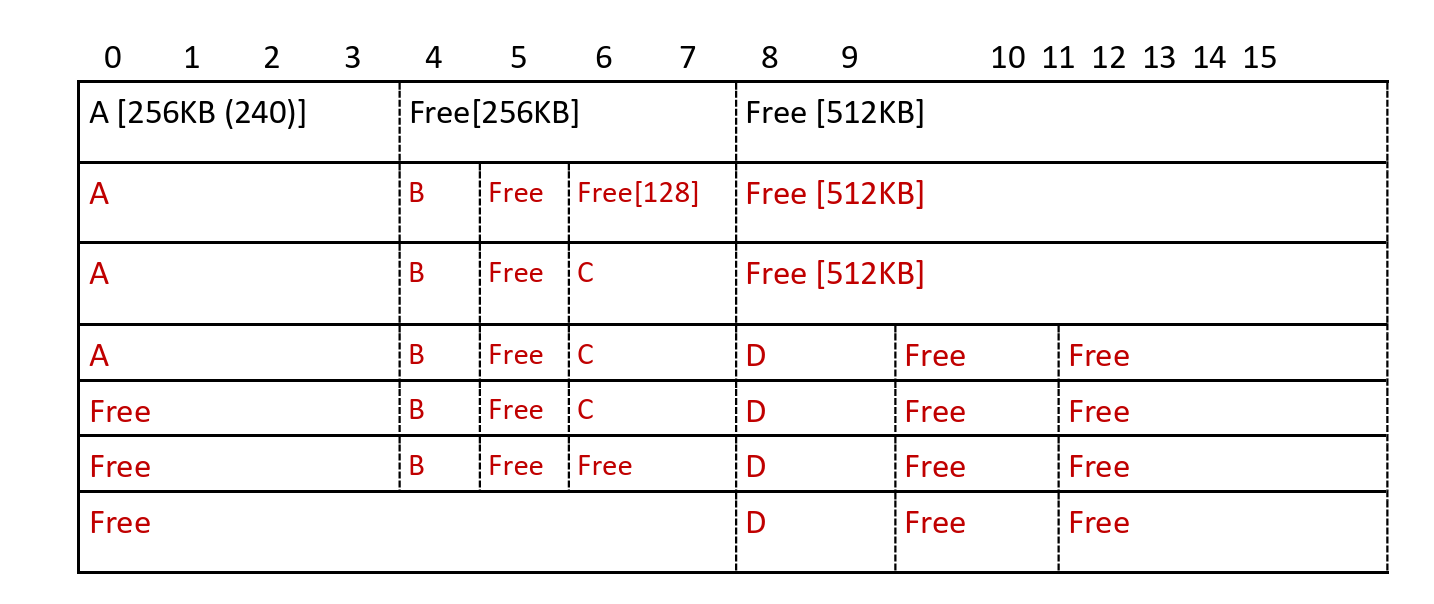
\includegraphics[width=1\linewidth]{images/final/1.png}
    \begin{itemize}
        \item \textbf{Allocation}: Find the smallest available block that fits the process, recursively splitting larger blocks into two equal-sized buddies until that smallest block is in our layout.
        \item \textbf{Deallocation}: Free the block and recursively merge it with its buddy if the buddy is also free. (Might have issue if two blocks are same size but are not buddy, so cannot be merged!)
        \item In \textbf{Buddy Allocation}, if no sufficiently large, properly aligned power-of-two block is available, the allocation fails. Just move on to do the next allocation!
    \end{itemize}
    \item In the buddy system, the min fragmentation is 0\% while the maximum fragmentation is about 50\%. At most 50\% of blocks of size $2^{N-1}$ are free at any point of time. 
    \item \textbf{Buddy Blocks}: Convert both starting addresses to binary. They are buddies iff they differ by exactly one bit at position $k$ (counting from 0 at the right), and all lower bits are 0. Each block has size $2^k$ allocation units before merging (assume the LSB position is 0).
\end{enumerate}

\section{Disjoint Memory Schemes}
\begin{enumerate}
    \item Pay Attention when converting 2KB to binary numbers!
    \item (\textbf{Paging}):
    \begin{itemize}
        \item Divides the physical and logical memory into fixed-size pages and frames, respectively
        \item \textbf{Address Translation (Paging)}: Logical Address = $\langle P,D\rangle$.
        \begin{itemize}
            \item Split the logical address into \textbf{page number P} and \textbf{offset D}.
            \item Use \textbf{P} to index the page table and retrieve the physical frame number \textbf{F}.
            \item Calculate the physical address: $PA = F \times \text{Page Size} + D$.
        \end{itemize}
        \item Incorrect memory access is not catchable if it is still within valid page boundary. (Tut 8 Q1)
        \item The worst case memory access time is TLB miss + page table + page fault (two disk I/O as page might be dirty).
        \item In a two-level paging scheme, if a lower-level page table is itself not resident in RAM, accessing it may cause an additional page fault. Therefore, under this assumption, two or more page faults may occur: one for the missing page-table page and another for the requested data page, potentially requiring four secondary storage accesses in total.
        \item The cache is checked only after the virtual-to-physical address translation has been resolved (a.k.a, all the page fault has been resolved!).
    \end{itemize}
    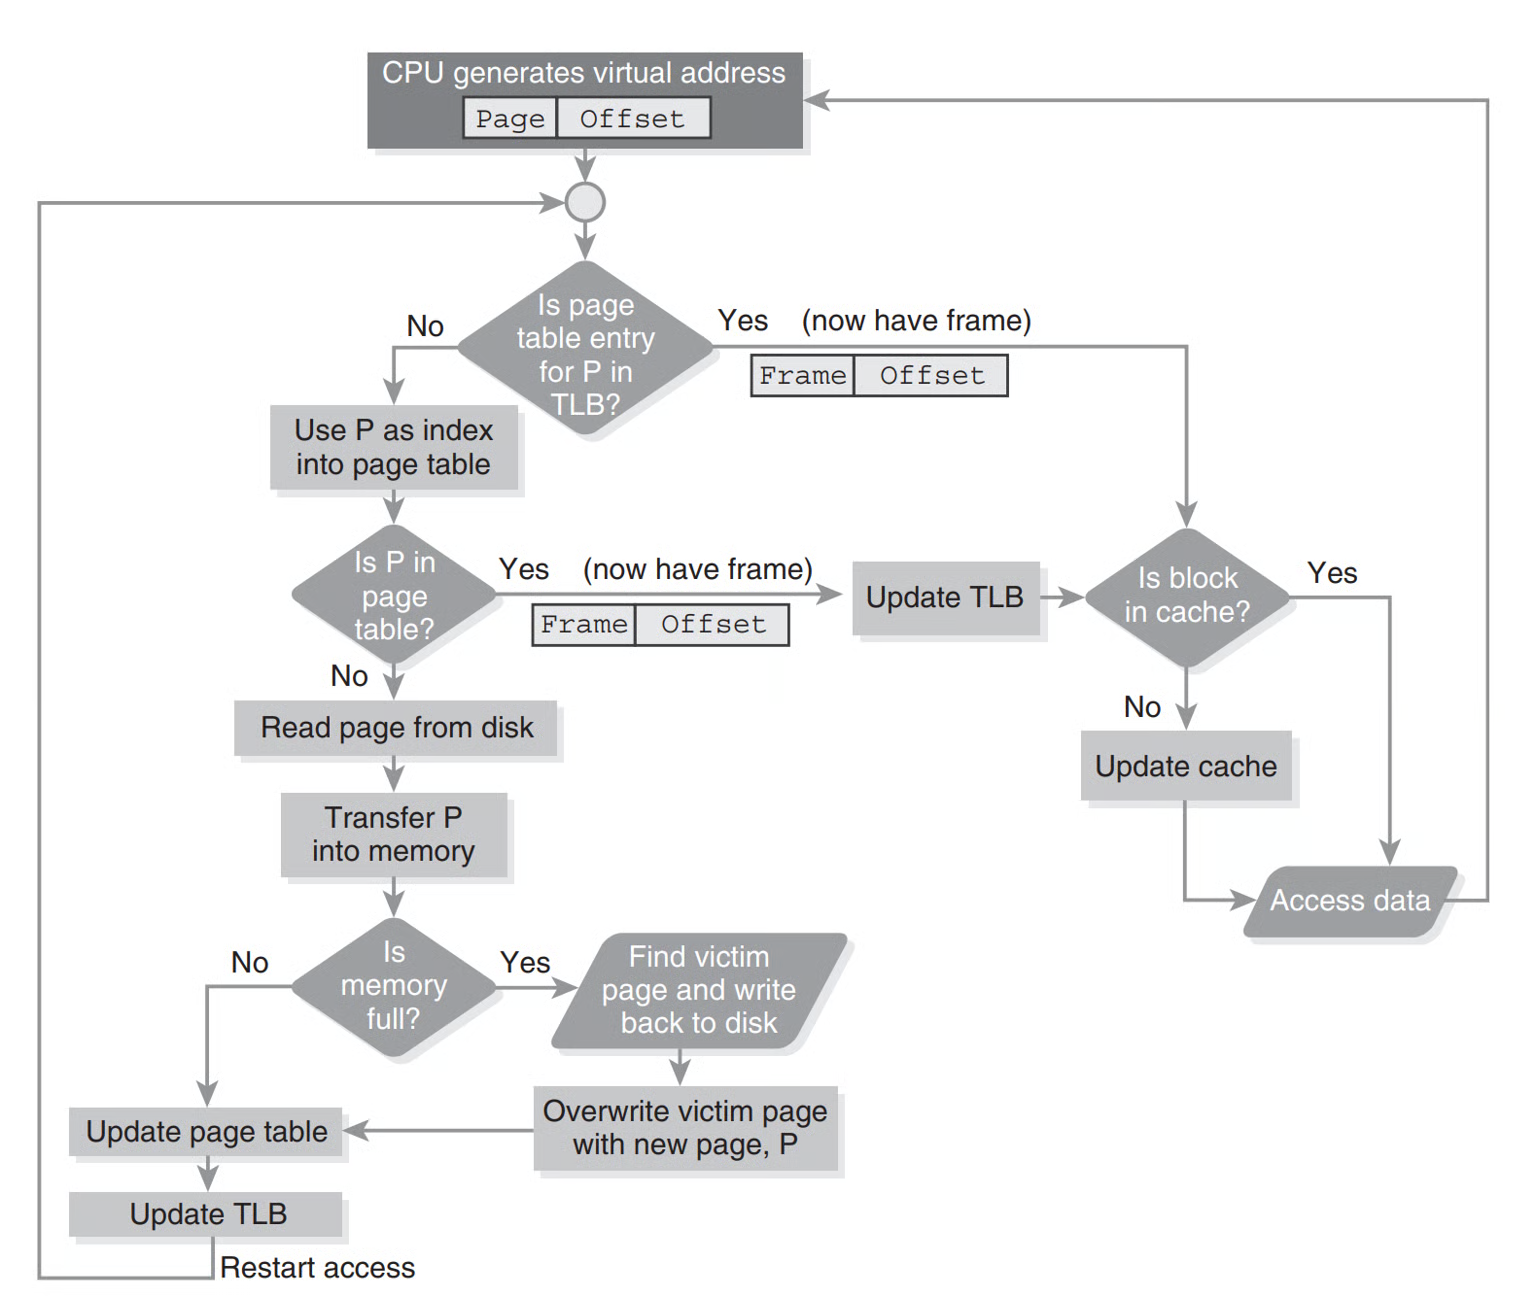
\includegraphics[width=1\linewidth]{images/final/2.png}
    \item (\textbf{Segmentation}):
    \begin{itemize}
        \item Each segment (e.g, code, heap, stack, data region of a process) must be mapped to a contiguous region of physical memory.
        \item \textbf{Address Translation}: $\text{Logical Address}=\langle\text{SegID},\text{Offset}\rangle$
        \begin{itemize}
            \item Use the \textbf{SegID} to look up the \textbf{base} and \textbf{limit} in the segment table.
            \item Check the offset: if $\text{Offset} < \text{Limit}$, the access is valid; otherwise, an addressing error occurs.
            \item Calculate the physical address: $\text{PA} = \text{Base} + \text{Offset}$.
        \end{itemize}
        \item Generally, segmentation suffers from \textbf{external fragmentation} but no internal fragmentation.
    \end{itemize}
    \item (\textbf{Segmentation with Paging})
    \begin{itemize}
        \item Each process is still divided into segments, such as Code, Data, etc. Each segment is further divided into fixed-size pages and has its \textbf{own page table}. The pages of each segment can be stored in \textbf{non-contiguous physical frames}.
        \item \textbf{Address Translation}: $\text{Logical Address}=\langle S,P,D\rangle$, $S$ denotes Seg ID, $P$ denotes page number and $D$ denotes offset.
        \begin{itemize}
            \item Use \textbf{S} to look up the segment table for the \textbf{page limit} and \textbf{page table base}.
            \item Check if $P < \text{Page Limit}$; otherwise, an addressing error occurs.
            \item Use \textbf{P} to index the segment's page table and retrieve the physical frame number \textbf{F}.
            \item Calculate the physical address: $PA = F \times \text{Page Size} + D$.
        \end{itemize}
        \item Segmentation determines which page table to use, while paging determines which physical frame contains the requested page.
        \item This scheme only suffers from internal fragmentation in the last page.
    \end{itemize}
    \item Most importantly, before applying paging, segmentation, or their combination, always write out the data in its \textbf{original sequential order in logical memory}! This makes it much easier to identify the correct page numbers, segment numbers, and offsets when performing address translation.
    \item Page table and segmentation table usually stays in the main memory.
    \item Each process has its own page table! But the TLB is a hardware cache \textbf{shared across processes} running on the same CPU core
    \item The TLB resides in cache and each TLB entry holds a virtual page number and its corresponding physical page number.
    \item Segmentation Table and Page Table example: \\
    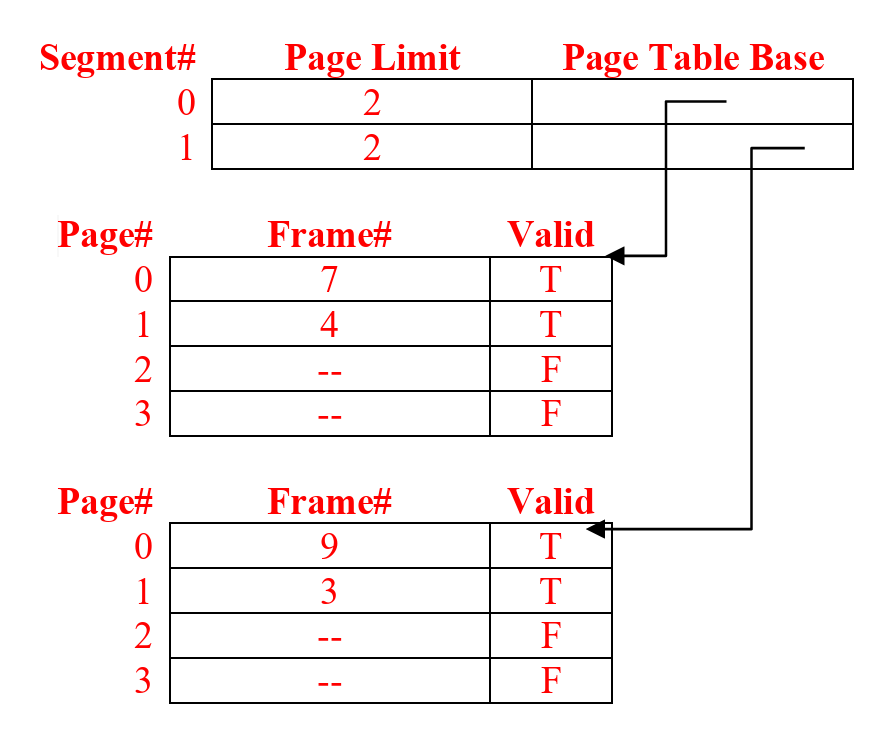
\includegraphics[width=1\linewidth]{images/final/3.png}
    \item The \textbf{Page Table Entry (PTE) width} can be derived from the number of bits required: physical frame number bits + additional control bits (e.g., valid/present, dirty, protection), depending on the question. Note that if the question specifies the PTE width, use that one!
    \item During a context switch, the OS locates the incoming process's page table and updates the \textbf{Page Table Base Register (PTBR)} accordingly. In the basic model, the TLB is also flushed. However, the outgoing process's page table does \textbf{not necessarily need to remain in physical memory}, as it may be swapped out.
    \item $\mathrm{KiB}=2^{10}$, $\mathrm{MiB}=2^{20}$, $\mathrm{GiB}=2^{30}$, and $\mathrm{TiB}=2^{40}$ bytes. In CG2271, KB=KiB.
\end{enumerate}

\section{Virtual Memory Management}
\begin{enumerate}
    \item The main point behind the two principles of localities is that: in a computer system, the memory access is \textbf{not random}!
    \item (\textbf{Demand Paging}): Instead of loading all pages before execution, only load pages into physical memory when they are needed (i.e., upon a page fault).
    \begin{itemize}
        \item \textbf{Demand Paging vs.\ Pre-paging}: Demand paging generally has a shorter \textbf{startup time} since pages are loaded only when accessed (causing initial page faults), whereas pre-paging loads several/all pages before execution, increasing startup time but reducing initial page faults. Note that startup time refers to the delay before execution begins, not the time to complete the first operation.
    \end{itemize}
    \item (\textbf{Inverted Page Table}): Maintains one table for the entire physical memory, indexed by the \textbf{physical frame number}, with each entry storing the \textbf{(PID, VPN)} pair.
    \begin{itemize}
        \item \textbf{Address Translation}: Logical Address = $(P,D)$; lookup key = $(PID,P)$.
        \begin{itemize}
            \item Obtain the \textbf{PID}, \textbf{VPN (P)}, and \textbf{offset (D)}.
            \item Search the inverted page table for an entry matching $(PID, P)$.
            \item If found at index $i$, the physical frame number is $F=i$.
            \item Calculate the physical address: $PA = F \times \text{Page Size} + D$.
        \end{itemize}
        \item \textbf{Inverted Page Table Memory}: A single system-wide table with one entry per physical frame. Thus, $\text{Total Size} = \text{Number of Physical Frames} \times \text{Entry Size}$.
    \end{itemize}
    \item (\textbf{Direct Paging}): 
    \begin{itemize}
        \item Calculate using the entire virtual address space. It's not the pages needed by the process(es)!!
    \end{itemize}
    \item (\textbf{Multi-level Page Table}): Since a process typically uses only a small portion of its virtual address space, we divide the original large page table into smaller page tables, indexed by higher-level page tables. This allows \textbf{only the required lower-level page tables to be allocated}, reducing the physical memory overhead.
    \begin{itemize}
        \item \textbf{Calculate the Number of Levels}: First, calculate the maximum PTEs per page table (we assume maximum one page per page table), $N = \frac{\text{Page Size}}{\text{PTE Size}}$. Then, repeatedly divide the total number of virtual pages by $N$ until the result is $\leq N$. The number of divisions plus one gives the required levels.
        \item Given the bit widths of a multi-level page table, we should be able to determine the page size ($2^{\text{offset bits}}$) and the number of entries per page table at each level ($2^{\text{index bits for that level}}$).
        \item \textbf{Calculate Physical Frames for Each Level (Tut 9 Q2, Important)}:
        \begin{itemize}
            \item \textbf{Step 1}: Split the virtual address into page-table indices and the page offset. The indices indicate which entry within the page table that the array starts, which may not be at entry 0.
            \item \textbf{Step 2 (Last Level)}: Calculate the number of virtual pages occupied by the array, accounting for the starting page offset. Each last-level PTE maps one virtual page. Since each page table holds at most $N$ entries, calculate the number of last-level tables needed, accounting for the starting index.
            \item \textbf{Step 3 (Higher Levels)}: Each higher-level entry points to one lower-level page table. Thus, the number of \textbf{entries} needed at the higher level equals the number of lower-level tables. Use this number of \textbf{entries} to calculate how many higher-level tables are required, accounting for the starting index at that level.
            \item \textbf{Step 4}: Repeat towards the root. Each allocated page table occupies one physical frame except for the root sometimes.
        \end{itemize}
        \item For a 1 GiB array, with 4 KiB pages and $N=512$ entries per page table (each PTE is 8 bytes) assume the start index is not 0 at the last-level page table:
        \begin{tabular}{|c|c|c|}
        \hline
        \textbf{Level} & \textbf{Entries Needed} & \textbf{Frames Needed} \\ \hline
        L4 (Last) & $2^{18}+1=262145$ & 513 \\ \hline
        L3 & 513 & 2 \\ \hline
        L2 & 2 & 1 \\ \hline
        L1 (Root) & 1 & 1 \\ \hline
        \end{tabular}
        \item Calculate Total Memory for Multi-level Page Tables: Each allocated page table (including the root) occupies one physical frame. Thus, $\text{Total Size} = \text{Total Frames} \times \text{Frame Size}$.
        \item In multi-level paging, the \textbf{root page directory does not necessarily occupy one full page}. Its size depends on the number of root entries, while lower-level page tables typically occupy one page each.
    \end{itemize}
    \item The Effective Memory Access Time (EMAT): $T_{\text{access}}=(1-p)T_{\text{mem}}+pT_{\text{page fault}}$, where $p$ is the probablity of page fault, which is $1-\text{Page Hit Rate}$.
    \begin{itemize}
        \item When calculating the memory access time for a page fault, remember to include the \textbf{TLB lookup} and the \textbf{final memory access} to retrieve the actual data. For example, with 4-level paging and a TLB miss, accessing a page whose page tables are in memory requires 1 TLB lookup + 5 main memory accesses (4 for page table traversal + 1 for data).
        \item For effective/average memory access time calculations involving TLB, cache, and page faults, calculate the average TLB and cache access times separately, then add the expected page fault penalty. If the page fault rate is conditional on a TLB miss: $ T_{\text{access}} =T_{\text{TLB,avg}}+T_{\text{cache,avg}}+P(\text{TLB miss})P(\text{fault}\mid\text{TLB miss})T_{\text{fault penalty}}$, where the $T_{\text{mem}}=T_{\text{TLB,avg}}+T_{\text{cache,avg}}$
        \begin{itemize}
            \item For each average access time calculation, we can use the EMAT formula.
            \item Whether after a cache miss or TLB miss, we will have to read the cache or TLB again will depend on the question!
        \end{itemize}
    \end{itemize}
    \item (OPT Page Replacement): \\
    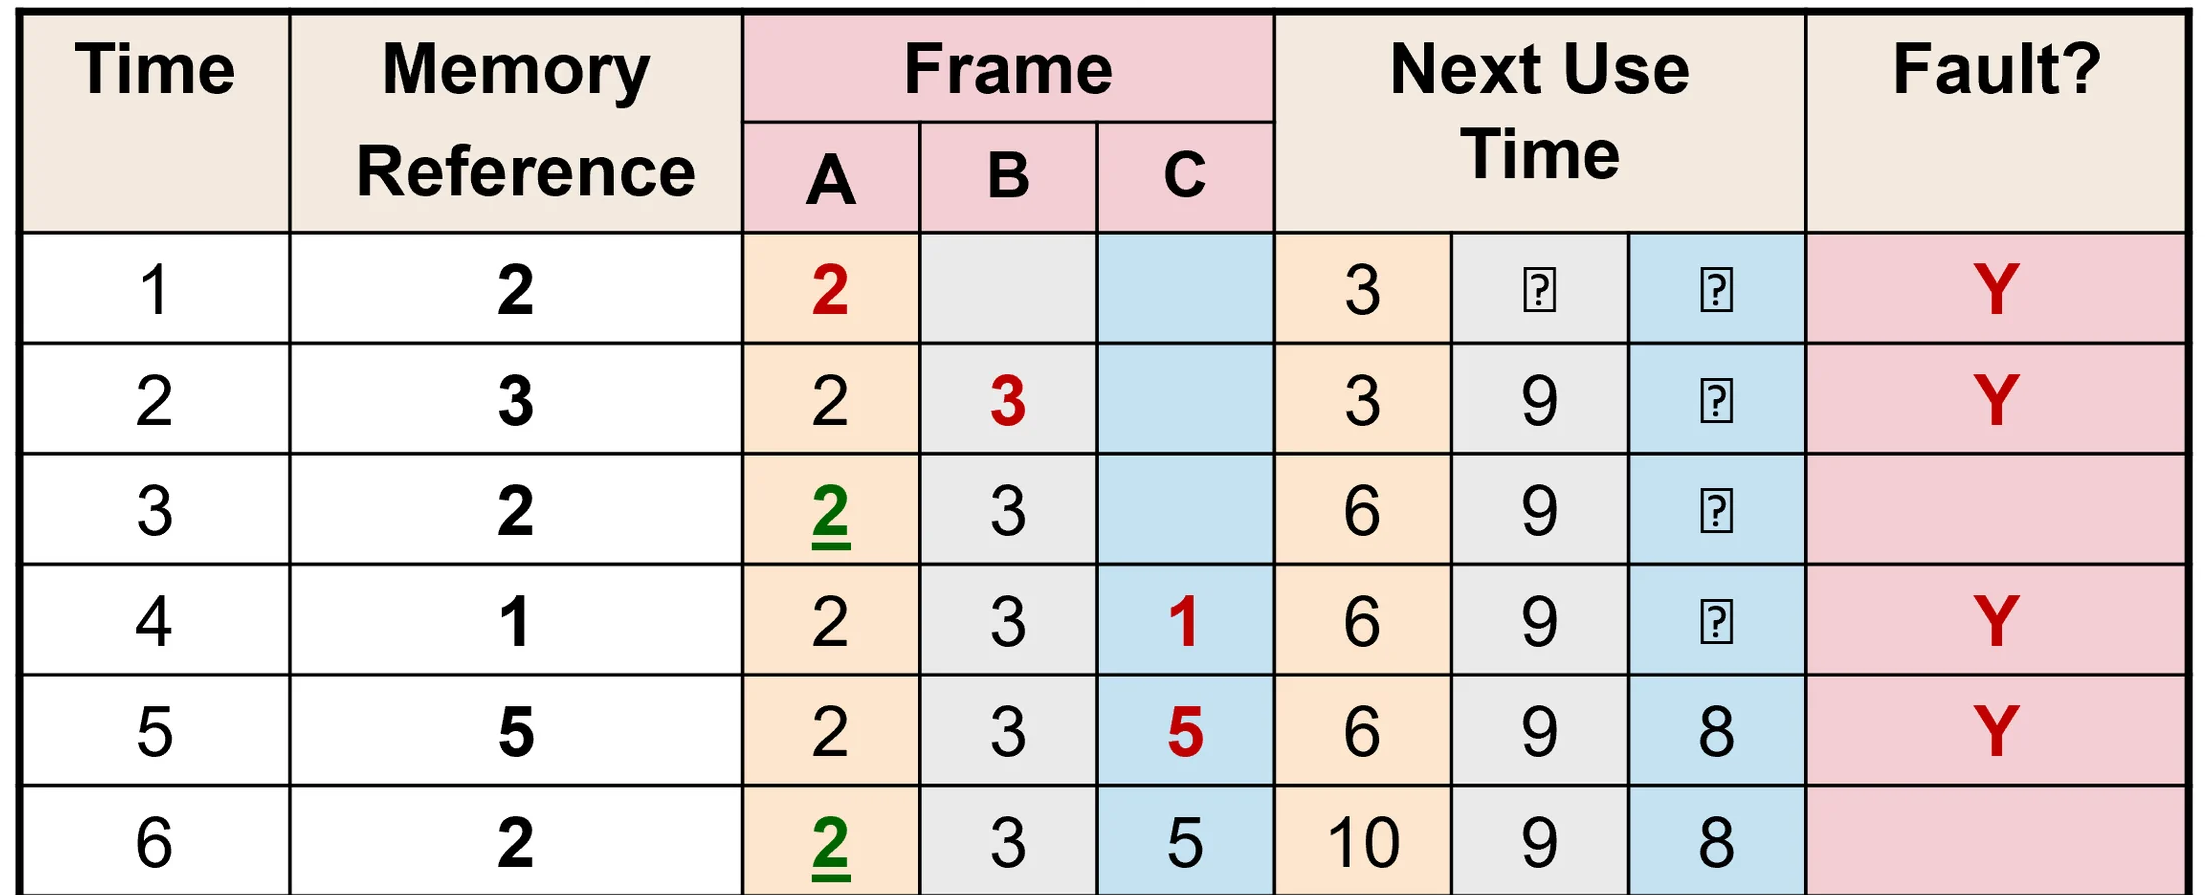
\includegraphics[width=1\linewidth]{images/final/7.png}
    \item (FIFO Page Replacement): It performs bad because it doesn't consider the temporal locality rule. \\
    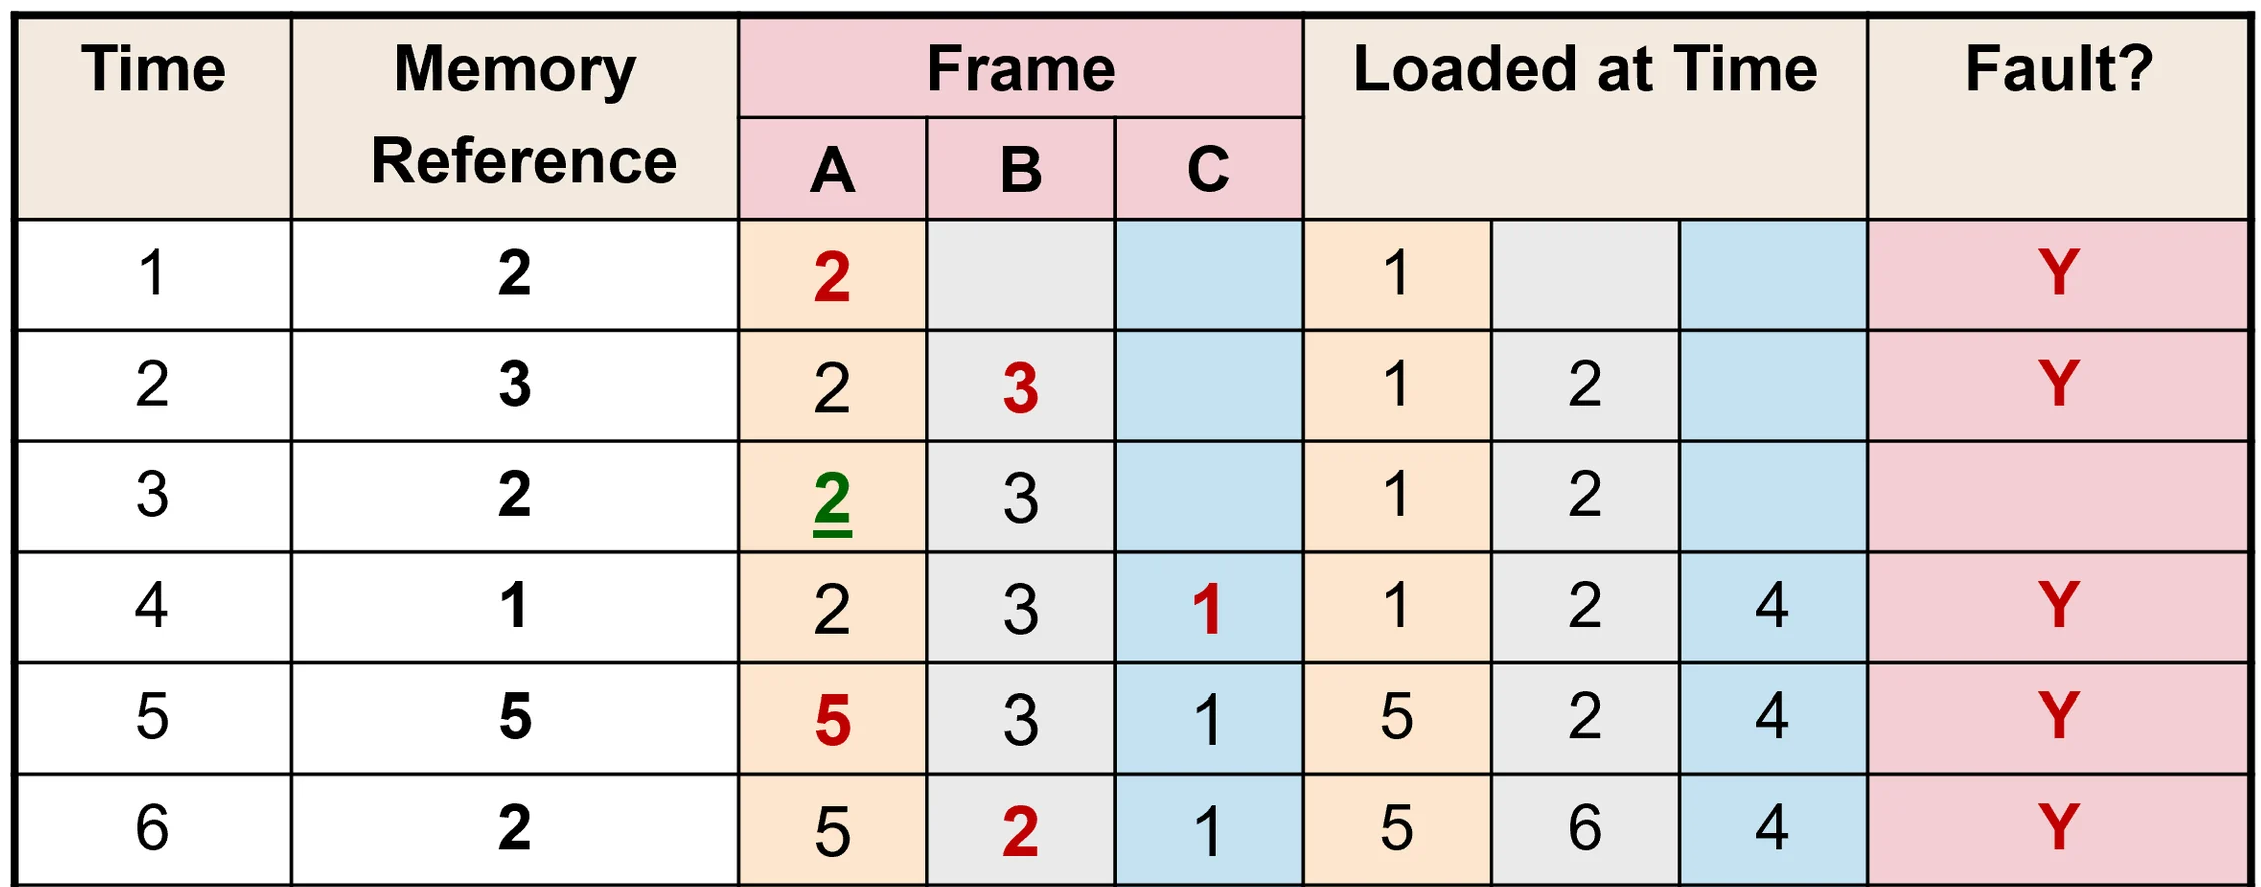
\includegraphics[width=1\linewidth]{images/final/8.png}
    \item (LRU Page Replacement): Evict the page that \textbf{has not been} accessed for the longest period of time.\\
    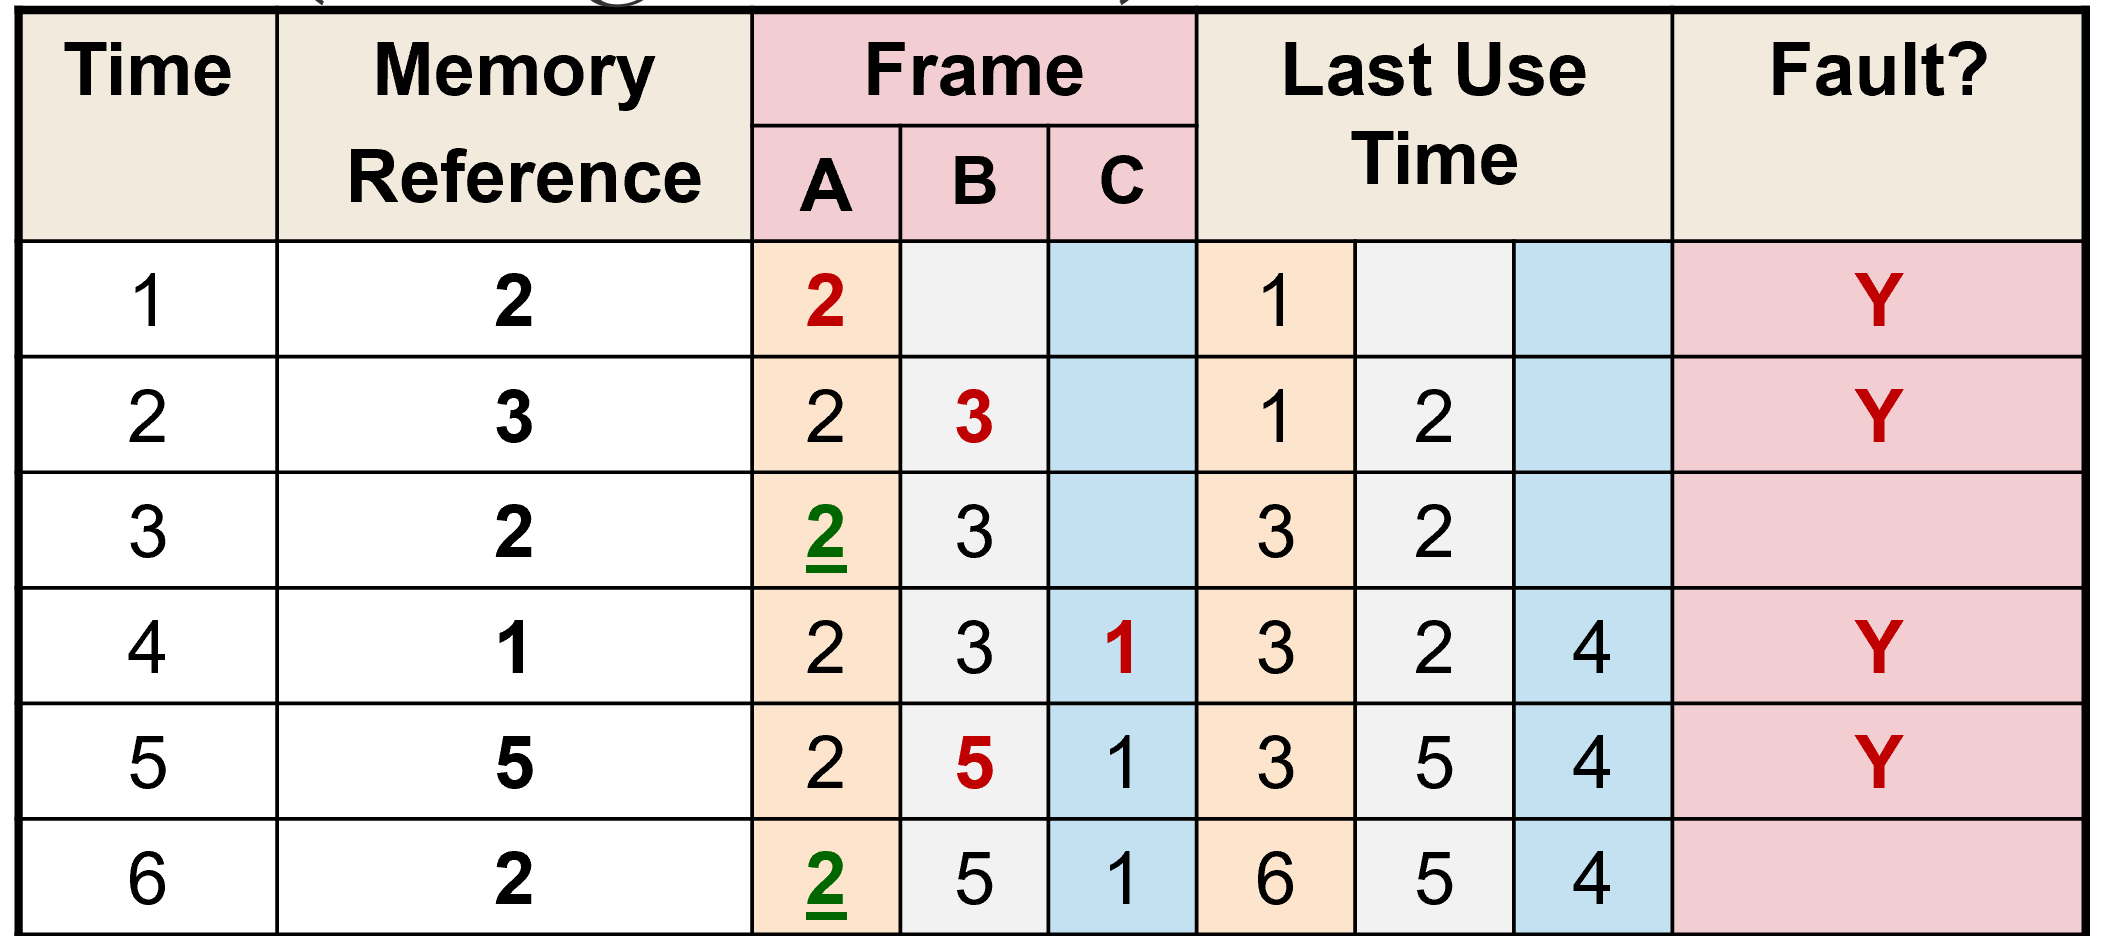
\includegraphics[width=1\linewidth]{images/final/9.png}
    \item \textbf{Second-Chance (Clock) Replacement}: Approximates \textbf{LRU} using a circular list of frames (a clock pointer) and a reference bit $R$.
    \begin{enumerate}
        \item Check the frame pointed to by the \textbf{clock pointer}:
        \begin{itemize}
            \item If $R=0$: Evict the page and replace it with the requested page.
            \item If $R=1$: Give it a second chance by setting $R=0$ and advancing the pointer.
        \end{itemize}
        \item Repeat until a frame with $R=0$ is found.
        \item After replacement, advance the clock pointer to the next frame.
    \end{enumerate}
    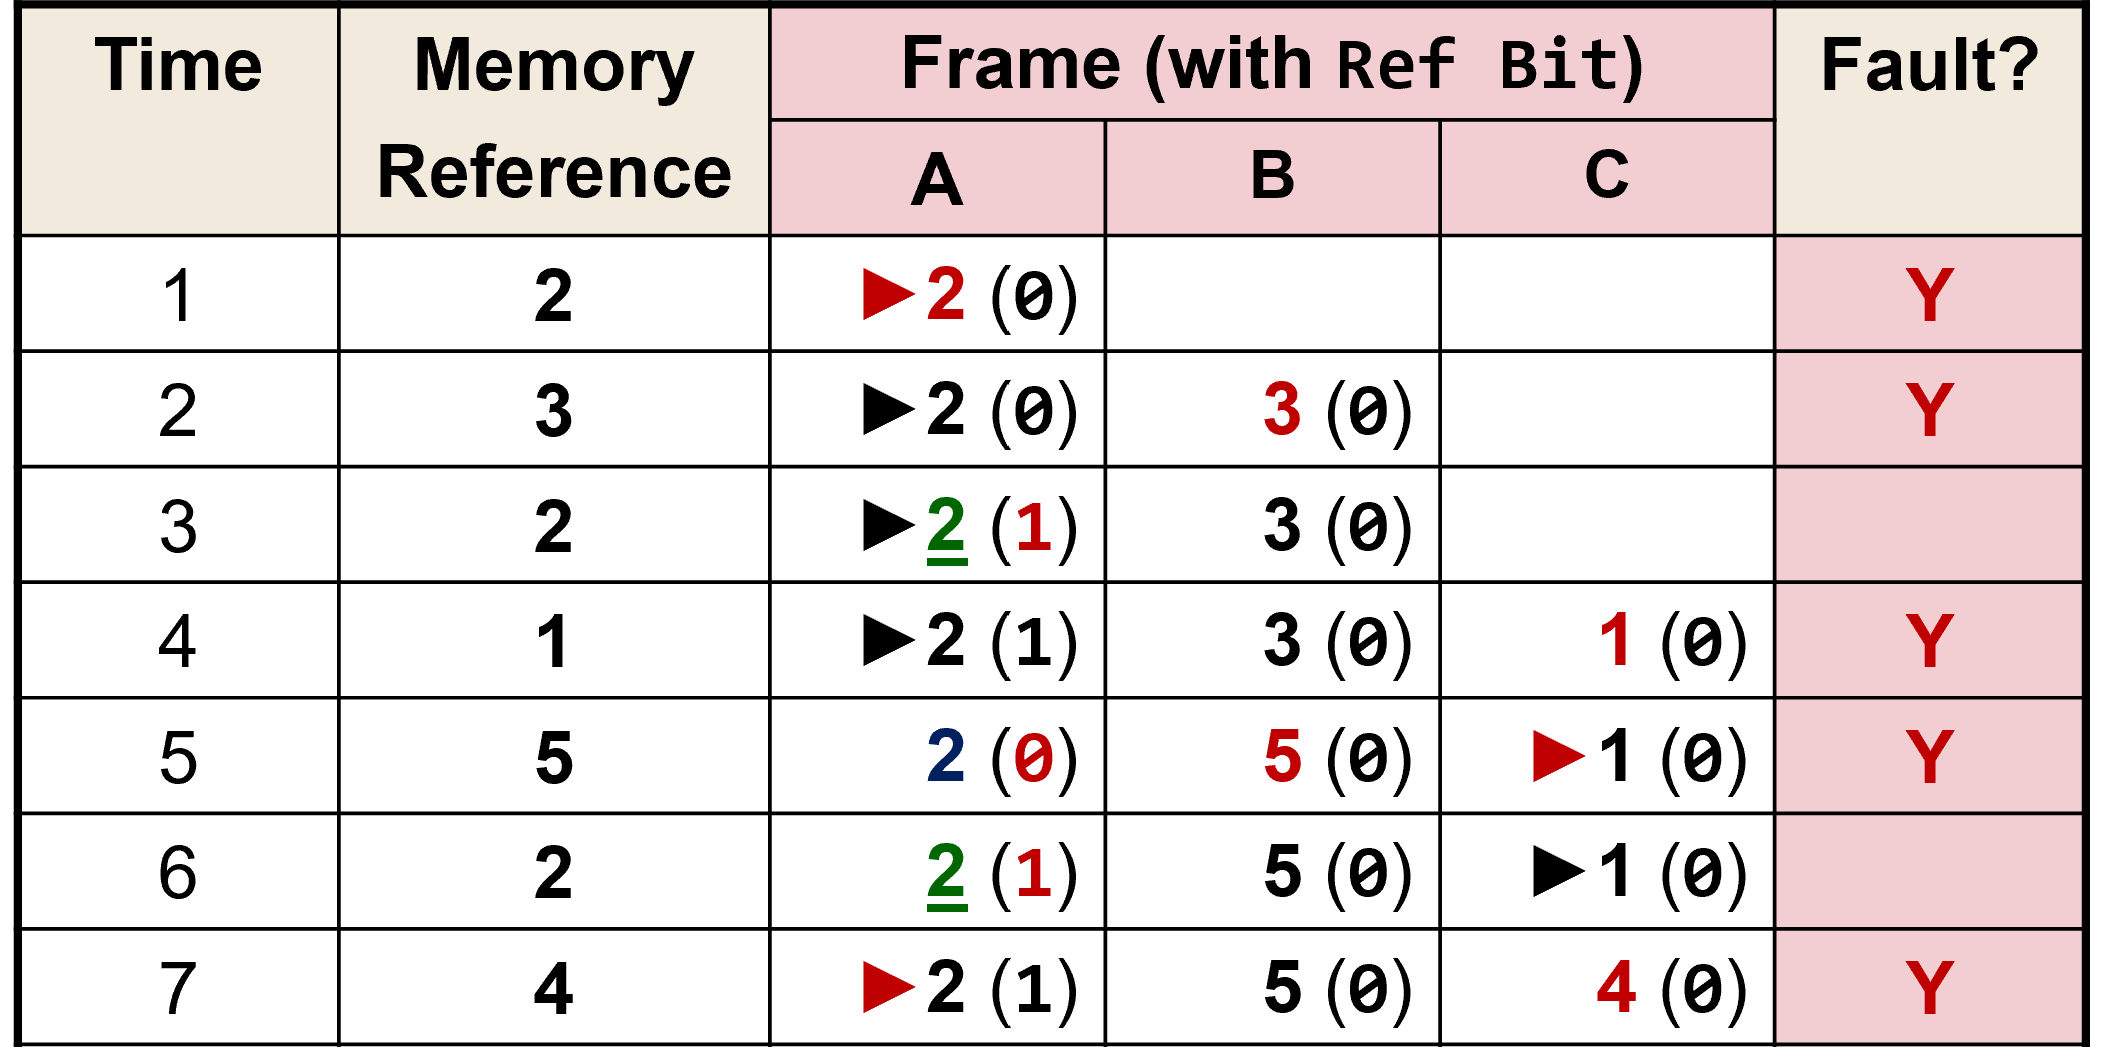
\includegraphics[width=1\linewidth]{images/final/10.png}
    \item Frame allocation determines how many \textbf{physical frames} are actually allocated to a process.
    \item The working set at time $t$, denoted by $W(t,\Delta)$, is the set of \textbf{distinct pages} referenced within the most recent $\Delta$ memory references.  \\
    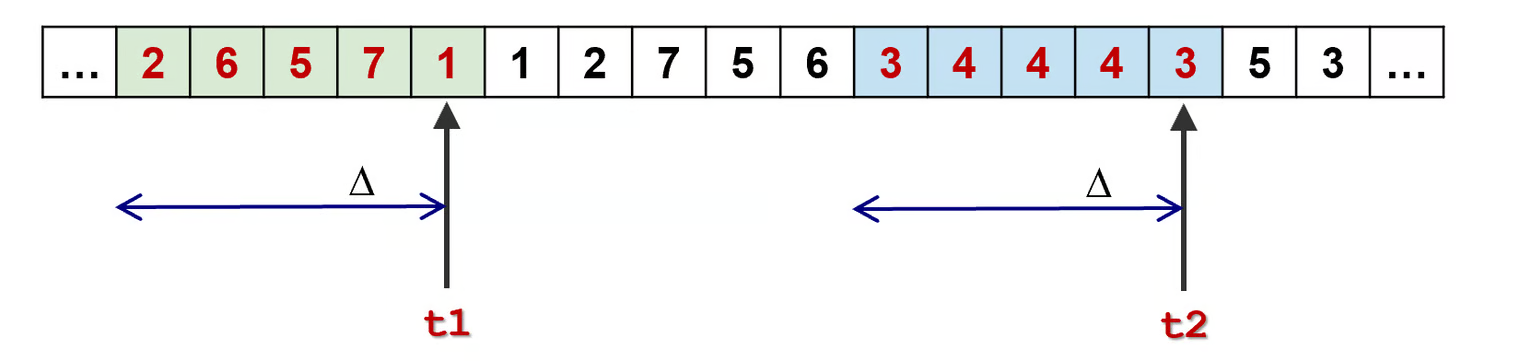
\includegraphics[width=1\linewidth]{images/final/4.png}
    \begin{itemize}
        \item In practice, $\Delta$ is chosen arbitrarily, although it has a huge impact.
        \item In the example above, $W(t_1,\Delta)=\{1,2,5,6,7\}$ (5 Frames needed). $W(t_1,\Delta)=\{3,4\}$ (2 frames needed).
        \item The working set model is one approach used by the OS to implement \textbf{dynamic frame allocation} (allocate physical frames to a process based on its actual need)
    \end{itemize}
\end{enumerate}

\section{File System Introduction}
\begin{enumerate}
    \item Each process maintains a \textbf{per-process open-file table}, implemented as an array indexed by file descriptors which is just an integer serving as an index into the \textbf{per-process open-file table}. Each entry points to an open-file object in the system-wide open-file table. The open-file object is \textbf{per-open}, not per-file! \\
    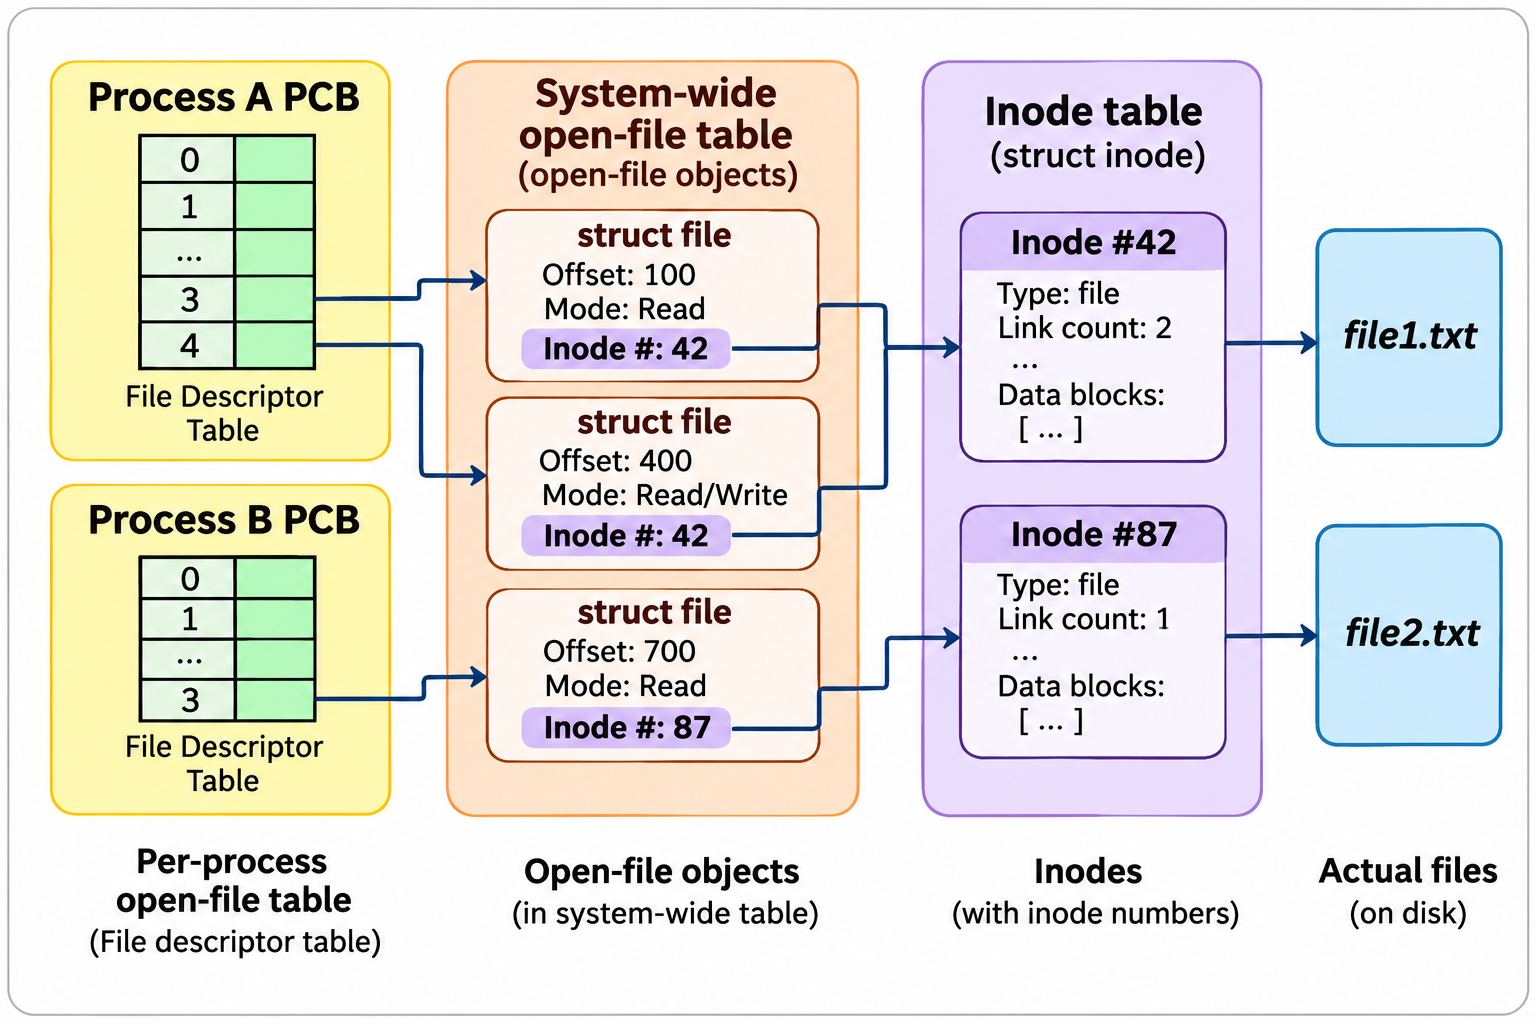
\includegraphics[width=1\linewidth]{images/final/5.png}
    \item \textbf{File Descriptors after \texttt{fork()}}: The parent and child have separate file descriptor tables, but inherited descriptors point to the \textbf{same open-file entry}, sharing the file offset and status flags.
    \item (\textbf{Hard link}): A \textbf{hard link} creates another directory entry (filename) that refers to the \textbf{same underlying file}, meaning that both filenames share the \textbf{same inode number}.
    \item A \textbf{symbolic link (soft link)} is a special type of file that stores the \textbf{pathname of another file or directory}, rather than directly referencing its inode.
    \begin{itemize}
        \item Symbolic links can therefore create \textbf{cycles} during pathname traversal.
    \end{itemize}
    \item If a file is currently being written by Process B, other processes (e.g., Process A) can generally still open the same file. However, the OS may provide file-locking or exclusive-access mechanisms to restrict concurrent access.
\end{enumerate}

\section{File System Implementation}
\begin{enumerate}
    \item (\textbf{Inode vs. Inode Table}): Each file or directory is associated with an inode number, which identifies its inode within the file system. The distinction is simple: the inode number is an index used to locate an entry in the inode table, while the inode is the actual data structure stored at that entry, containing the file's metadata. The inode table is just a bunch of inodes.
    \item In an inode-based file system, the \textbf{maximum number of partition blocks} is determined by the block pointer width ($2^{\text{pointer bits}}$), the \textbf{maximum number of files} by the number of available inodes, and the \textbf{maximum file size} by the inode's direct and indirect pointer structure.
    \item Each inode is identified by an inode number (i-number), given an inode number, the file system can directly calculate the on-disk location of the corresponding inode, without searching through the inode table. \\
    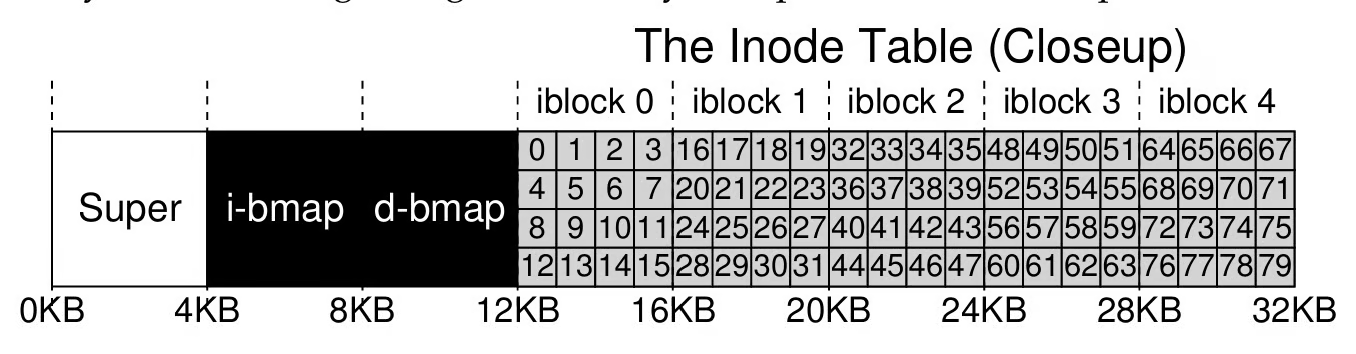
\includegraphics[width=1\linewidth]{images/final/6.png}
    \item Each inode will store the metadata of a file, one very important metadata is the \textbf{data block pointer}, where each pointer contains the disk address of a data block belonging to the file. Multi-level indexing can also be applied here so that now instead of pointing to a block that contains user data, it points to a block that contains more pointers, each of which point to user data.
    \begin{itemize}
        \item The sequence of imbalanced data pointer: Direct $\rightarrow$ singly indirect $\rightarrow$ doubly indirect $\rightarrow$ triply indirect.
    \end{itemize}
    \item The directory itself has an inode stored in the inode table, which contains metadata and pointers to its data blocks. The key difference is that a \textbf{directory's data blocks} store a list of \textbf{directory entries} (files or other directories), each mapping a filename to its corresponding inode number.
    \item Read \texttt{/foo/bar} timeline using inode. \\
    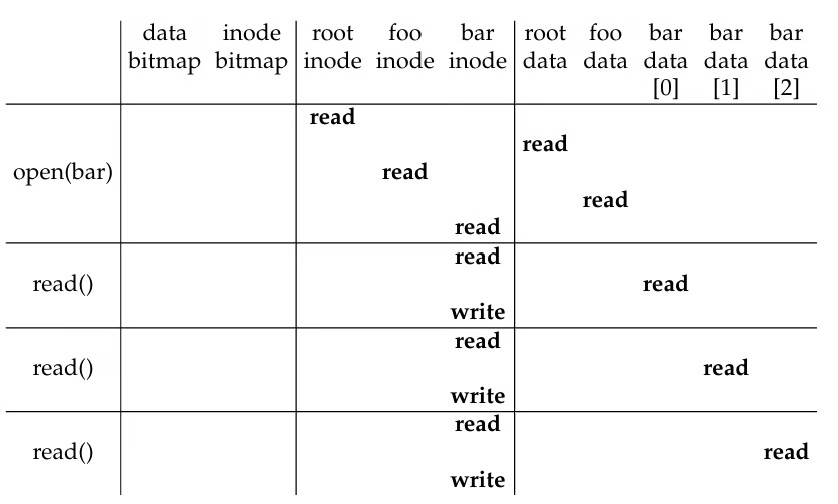
\includegraphics[width=1\linewidth]{images/final/11.png}
    \item Write \texttt{/foo/bar} timeline using inode \\
    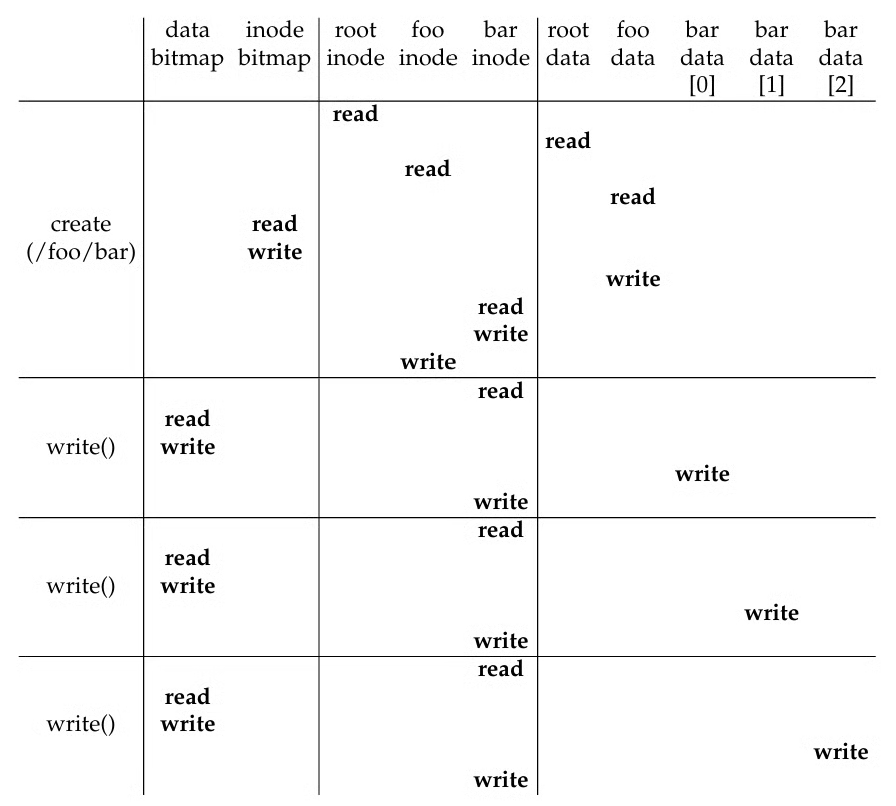
\includegraphics[width=1\linewidth]{images/final/12.png}
    \item Besides inode file blocks allocation, we also have \textbf{linked list} and \textbf{improved linked list} (FAT) allocation.
    \begin{itemize}
        \item \textbf{Linked Allocation}: Each data block stores both the file data and a pointer to the next block. Random access is inefficient because the blocks must be traversed sequentially.
        \item \textbf{FAT}: Stores the next-block pointers in a separate File Allocation Table, typically cached in memory. This improves random access compared to linked allocation, although traversing the FAT chain is still required.\\
        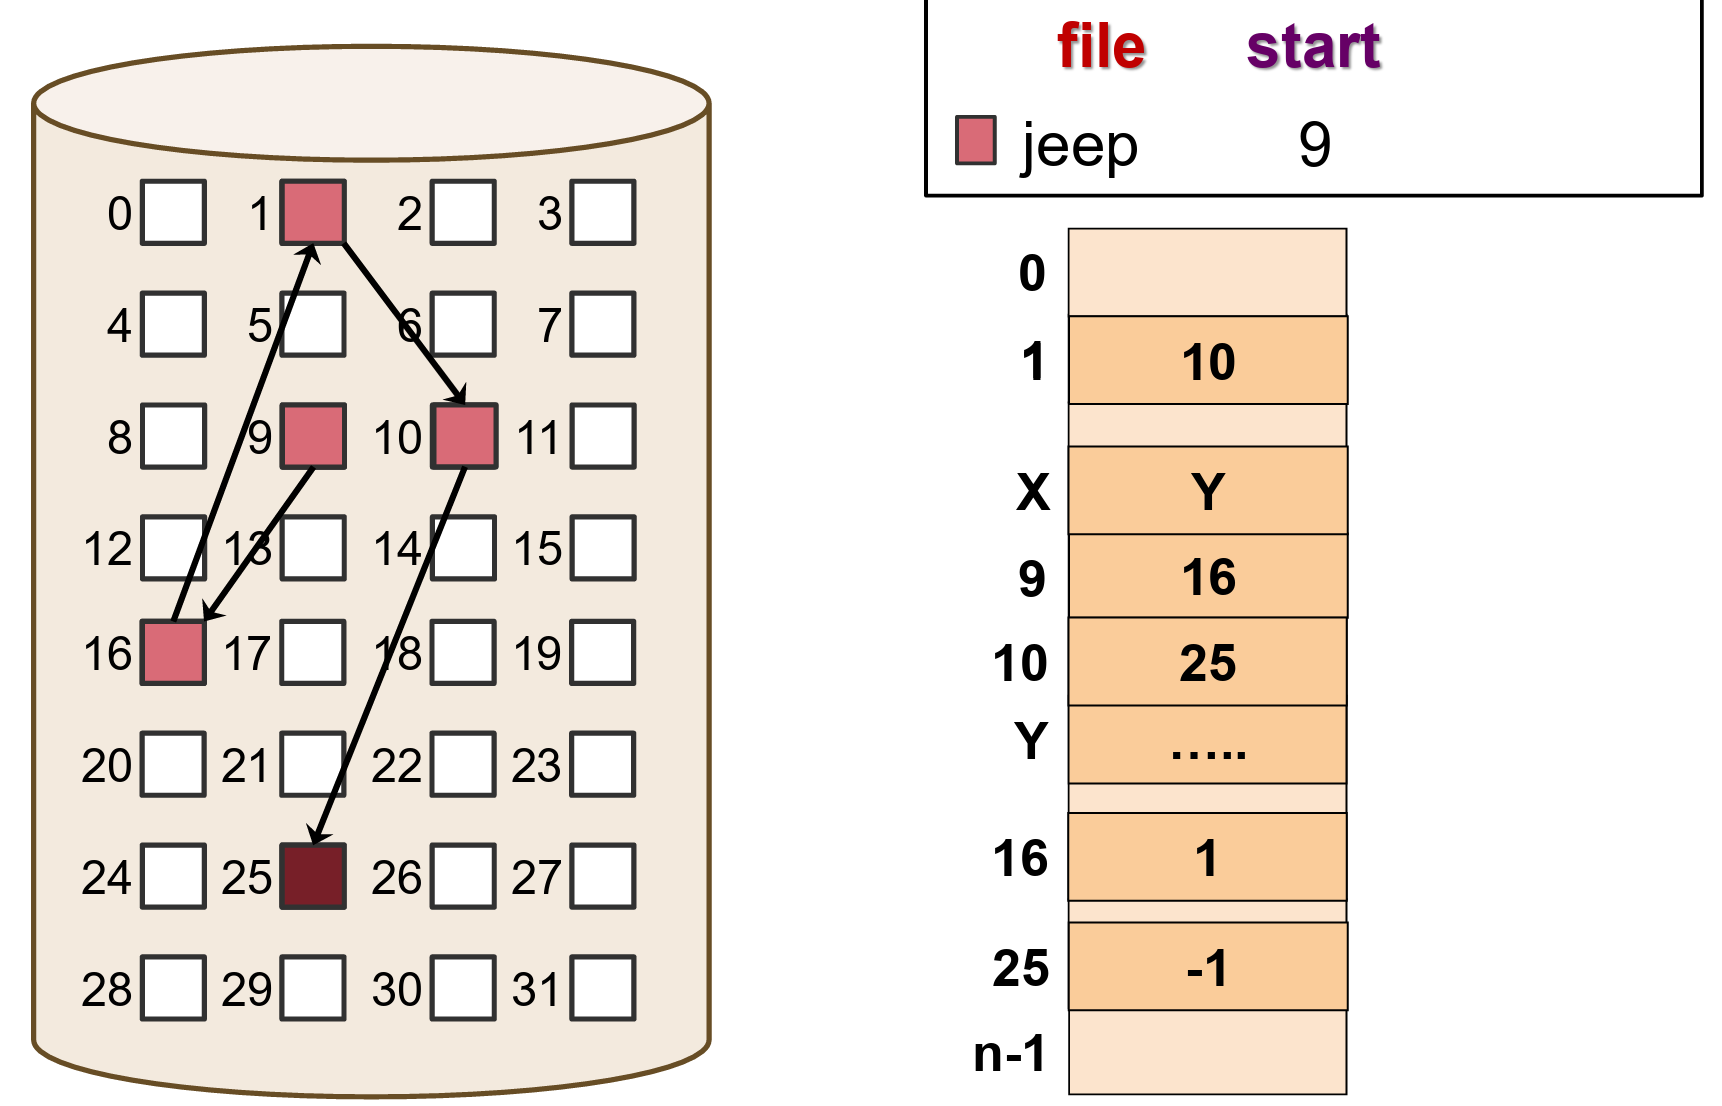
\includegraphics[width=1\linewidth]{images/final/13.png}
    \end{itemize}
    \item (HDD Basics)
    \begin{itemize}
        \item \textbf{HDD Structure}: Data is stored on tracks divided into sectors. The disk head moves between tracks (seek), while the disk rotates to access different sectors.
        \item \textbf{Disk Access Time}: $T_{\text{access}} = T_{\text{seek}} + T_{\text{rotation}} + T_{\text{transfer}}$.
        \item \textbf{Seek Time}: Time to move the disk head to the desired track (typically 2--10 ms).
        \item \textbf{Rotational Latency}: Time for the desired sector to rotate under the head. Average latency is half a rotation: $T_{\text{rotation,avg}} = \frac{60}{2 \times \text{RPM}}$ seconds. Transfer time is $\frac{\text{Data Size}}{\text{Transfer Rate}}$, usually much smaller.
        \item \textbf{Disk Scheduling}: The OS schedules I/O requests mainly to reduce seek time. Algorithms include FCFS (arrival order), SSF (nearest track first), and SCAN (head moves back and forth across tracks).
    \end{itemize}
\end{enumerate}

\section{Miscs}
\begin{enumerate}
    \item \textbf{True}:
    \begin{itemize}
        \item FAT provides a good method by which to  access to random access in files.
        \item User-level threads cannot be scheduled by the kernel
        \item Managing contiguous memory using linked-lists is generally faster than using bitmaps.
        \item A contiguous system with 1-byte allocation unit has no internal fragmentation.
    \end{itemize}
    \item \textbf{False}:
    \begin{itemize}
        \item Shared-variable access always requires mutual exclusion. (Not every access creates a race condition)
        \item FCFS works very well for I/O-bound tasks. (I/O bound tasks must wait for the CPU-bound tasks to finish, this is called convoy effect).
        \item A contiguous system with 1-byte allocation unit has no external fragmentation.
        \item Expanding one segment in pure segmentation requires relocation of the entire process if no adjacent free space exists (only affect segments need to be reallocated)
    \end{itemize}
\end{enumerate}

\end{multicols}

% Dividing Line
% \hrulefill \\
% \begin{multicols}{4}
% \begin{enumerate}
% \end{enumerate}
% \end{multicols}

\end{document}